\documentclass[a4paper,12pt]{article}
\usepackage{times}
\usepackage{parskip}
\usepackage{subcaption}
\usepackage[font=footnotesize]{caption}
\usepackage{tabularx}
\usepackage{graphicx}
\usepackage{amsmath}
\usepackage{fancyhdr}
\usepackage[headheight=15pt, margin=1in]{geometry}
\usepackage{fourier}
\usepackage{float}
\usepackage{multirow}
\usepackage{cite}
\usepackage{diagbox}
\usepackage{booktabs}

\linespread{1.1}
% Configure paragraph spacing - no indentation, small space between paragraphs
\setlength{\parskip}{1em}  % Space between paragraphs
\setlength{\parindent}{0pt}  % No indentation

\title{Building a Neural Network Pipeline for Patch-Level Classification in Histopathology Whole-Slide Images}
\author{Estella Ge, Leo Qi, Tiger Ding}
\date{November 2025}

\pagestyle{fancy}
\fancyhf{}
\rhead{Page \thepage\ of \pageref{LastPage}}

% Begin document
\begin{document}

\maketitle
\thispagestyle{empty}
\clearpage

\tableofcontents
\thispagestyle{empty}
\clearpage

\setcounter{page}{1}
\pagestyle{fancy}

\section{Introduction}
\subsection{Background}
Histopathology remains the cornerstone of cancer diagnosis and patient management. However, the traditional clinical workflow, which relies on the manual examination of gigapixel-scale Whole-Slide Images (WSIs), is inherently labor-intensive and subject to significant inter-observer variability. As the digitization of pathology accelerates, producing data of increasing scale and resolution, there is a critical need for automated computational approaches. These systems are essential for augmenting the capabilities of pathologists, enhancing diagnostic efficiency, and ensuring consistent identification of morphological structures and cellular abnormalities.

To address these challenges, deep learning has emerged as a transformative tool in computational pathology. Early iterations of these pipelines predominantly relied on Convolutional Neural Networks (CNNs), such as ResNet and DenseNet, to perform patch-level classification. While these baselines established strong benchmarks for local feature extraction and accuracy \cite{kather_multi-class_2016}, their inductive bias towards local texture often limits their ability to model long-range dependencies and the broader spatial context of the tissue microenvironment.

More recently, the field has witnessed a paradigm shift toward Vision Transformers (ViTs) and large-scale foundation models. Architectures leveraging self-supervised learning objectives, such as DINO-based models, Virchow, and HistoMIL, have demonstrated superior generalization capabilities \cite{caron_emerging_2021,vorontsov_virchow_2024}. By utilizing self-attention mechanisms, these models effectively capture global tissue architecture and complex spatial relationships that often elude standard CNNs.

However, this performance advantage comes at a cost. The deployment of large transformer-based architectures demands substantial computational resources, raising significant concerns regarding their scalability and efficiency in high-throughput clinical settings. This trade-off necessitates a critical examination of modern pipeline design: specifically, whether complex, heavy-weight architectures are required for downstream tasks, or if the rich, high-dimensional semantic representations encoded by foundation models can be effectively exploited by more efficient, lightweight classifiers.

\subsection{Goal of Project}
The primary objective of this work is to develop a balanced and efficient workflow for patch-level histopathology classification that effectively integrates transformer-based representations with lightweight neural network architectures. Beyond implementation, we conduct a comprehensive comparative analysis of these models, evaluating them across key performance metrics including classification accuracy, computational cost, and operational practicality. This assessment is designed to inform the selection of optimal architectures for real-world applications, balancing the trade-offs between diagnostic precision and resource constraints.

\subsection{Related Works}
While standard CNN baselines have established a strong benchmark with accuracies ranging from 91\% to 94\% on the NCT-CRC-HE-100K dataset \cite{kather_predicting_2019}, emerging transformer-based foundation models have pushed these boundaries further. By leveraging pretraining on millions of histological tiles, these models report superior accuracies of 94\% to 97\% \cite{pan_histomil_2023}, effectively outperforming traditional architectures while significantly reducing the dependency on large, fully annotated datasets.

\subsection{What Our Project Will Do}
First, we will utilize pretrained CNN-based and ViT-based models to extract features from histopathology tiles. We aim to perform a two-fold comparison: distinctively analyzing Multiple Instance Learning (MIL) on ViT patch embeddings versus classifiers using ViT CLS tokens, while simultaneously benchmarking CNN architectures against ViT models regarding training times and other performance metrics. To achieve this, we will implement and compare four classifiers: \begin{enumerate} \item VGG-16 \item ResNet-50 \item PatchMIL (attention based aggregation of ViT patch embeddings) \item MulticlassMLP (efficient ViT CLS-token classifier) \end{enumerate} We will evaluate the models' performance on the NCT-CRC-HE-100K dataset, specifically analyzing error rates, computational efficiency, and suitability for clinical integration. Ultimately, we hope to determine the trade-offs between patch-level aggregation and token-based classification within ViT architectures, as well as how they compare to traditional CNN baselines.


\section{Methods}

\subsection{Dataset}
We utilized the NCT-CRC-HE-100K dataset, which comprises 100,000 non-overlapping image patches extracted from hematoxylin \& eosin (H\&E) stained histological whole-slide images of human colorectal cancer (CRC) and normal tissue \cite{kather_100000_2018}. All images are standardized at 224$\times$224 pixels with a resolution of 0.5 microns per pixel (MPP) and have been color-normalized using Macenko's method to ensure consistency across samples. The dataset encompasses nine distinct tissue classes: Adipose (ADI), background (BACK), debris (DEB), lymphocytes (LYM), mucus (MUC), smooth muscle (MUS), normal colon mucosa (NORM), cancer-associated stroma (STR), and colorectal adenocarcinoma epithelium (TUM). These patches were manually extracted from 86 H\&E stained human cancer tissue slides obtained from formalin-fixed paraffin-embedded (FFPE) samples from the NCT Biobank and UMM pathology archive, including CRC primary tumor slides, tumor tissue from CRC liver metastases, and non-tumorous regions from gastrectomy specimens to increase variability.

\subsection{Feature Extraction}
For feature extraction, we employed the Virchow2 model, a state-of-the-art vision transformer specifically designed for histopathology applications \cite{vorontsov_virchow_2024,zimmermann_virchow2_2024}. The Virchow2 model follows the ViT-H/14 architecture, containing 32 layers of transformer blocks and 16 attention heads \cite{dosovitskiy_image_2021}. It was loaded from the Hugging Face hub (paige-ai/Virchow2) with SwiGLUPacked MLP layers and SiLU activation functions. Each histopathology patch was processed through the model to generate comprehensive embeddings of dimension 261$\times$1280. The embedding structure is organized such that row 0 contains the CLS token embedding (for global image representation), rows 1-4 contain the register tokens, and rows 5-261 contain patch embeddings representing 256 localized 14x14 regions within each image. All embeddings were generated using mixed precision (float16) with automatic mixed precision and were saved incrementally as individual NumPy files to enable efficient storage and retrieval during training.

In addition to Virchow2, we also utilized CNN-based models including VGG-16 and ResNet-50 to extract image features from histopathology data. Compared to transformer architectures, CNNs such as VGG-16 and ResNet-50 are generally considered more lightweight and can offer faster model inference and training due to their efficient convolution operations and smaller parameter counts. These architectures have a long history of reliable performance in medical image analysis tasks, and their representations are well-suited for extracting localized texture features.

\subsection{Model Architectures}
We implemented four complementary neural network architectures for patch classification. The PatchMIL and MulticlassMLP models are built directly on the Virchow2 ViT embeddings generated during feature extraction, as described in the Feature Extraction section.

\subsubsection{PatchMIL Model}
The PatchMIL (Patch-based Multiple Instance Learning) model employs an attention mechanism to aggregate information from all the patch embeddings generated by feeding each image through Virchow2 \cite{vaswani_attention_2023}. The architecture consists of three main components: (1) An encoder network that processes individual patch embeddings through two sequential blocks with linear layers (input\_dim $\rightarrow$ 512 $\rightarrow$ 256), batch normalization, LeakyReLU activation ($\alpha$=0.1), and dropout (0.3, 0.4); (2) An attention mechanism that computes importance weights for each patch through a two-layer network (256 $\rightarrow$ 128 $\rightarrow$ 1) with tanh activation and softmax normalization across patches; and (3) A classifier network that processes the attention-weighted sum of patch features through two blocks (256 $\rightarrow$ 128 $\rightarrow$ 64 $\rightarrow$ num\_classes) with batch normalization, LeakyReLU activation, increasing dropout rates (0.4, 0.5), and a final linear output layer. During forward propagation, the model flattens patch embeddings, encodes them individually, computes attention weights, and produces a weighted aggregation of patch features before final classification.

\subsubsection{MulticlassMLP Model}
The MulticlassMLP model provides a more straightforward approach for image-level classification using the CLS token embedding from the Virchow2 outputs. This feedforward network consists of four sequential blocks: (1) Initial dimensionality reduction (input\_dim $\rightarrow$ 512) with batch normalization, ReLU activation, and 0.3 dropout; (2) Feature extraction (512 $\rightarrow$ 256) with batch normalization, ReLU activation, and 0.4 dropout; (3) Final feature refinement (256 $\rightarrow$ 128) with batch normalization, ReLU activation, and 0.5 dropout; and (4) Output layer (128 $\rightarrow$ num\_classes) producing class probabilities. The model operates directly on CLS token embeddings from the Virchow2 ViT, making it computationally efficient and suitable for scenarios requiring fast predictions, such as processing an entire whole-slide image.

\subsubsection{VGG-16 Classifier Model}
The VGG-16 classifier uses transfer learning to reduce training load and ensure better convergence on histopathology tasks. In our implementation, each image is passed through a VGG-16 backbone (pretrained on natural images), where the original classifier head is replaced with custom fully connected layers tailored for our target class labels. The VGG-16 architecture follows a sequential convolution pattern with progressive feature learning through five main blocks: (1) Two 3$\times$3 conv layers with 64 filters $\rightarrow$ 2$\times$2 max pooling; (2) Two 3$\times$3 conv layers with 128 filters $\rightarrow$ 2$\times$2 max pooling; (3) Three 3$\times$3 conv layers with 256 filters $\rightarrow$ 2$\times$2 max pooling; (4) Three 3$\times$3 conv layers with 512 filters $\rightarrow$ 2$\times$2 max pooling; (5) Three 3$\times$3 conv layers with 512 filters $\rightarrow$ 2$\times$2 max pooling; followed by adaptive average pooling. The custom classifier head consists of: (1) Linear(512$\times$7$\times$7 $\rightarrow$ 4096) + ReLU + Dropout(0.5) with 102,764,544 parameters; (2) Linear(4096 $\rightarrow$ 1024) + ReLU + Dropout(0.5) with 4,195,328 parameters; (3) Linear(1024 $\rightarrow$ 9) with 9,225 parameters for 9-class classification. The total parameter count is 121.7M with a memory footprint of approximately 596MB and computational complexity of 30.94 GFLOPs for forward pass. During training, we train both the feature extracting backbone and custom classifier head. The learning rate for the classifier head is higher than the backbone to match the two steps.

% \begin{figure}[H]
%     \centering
%     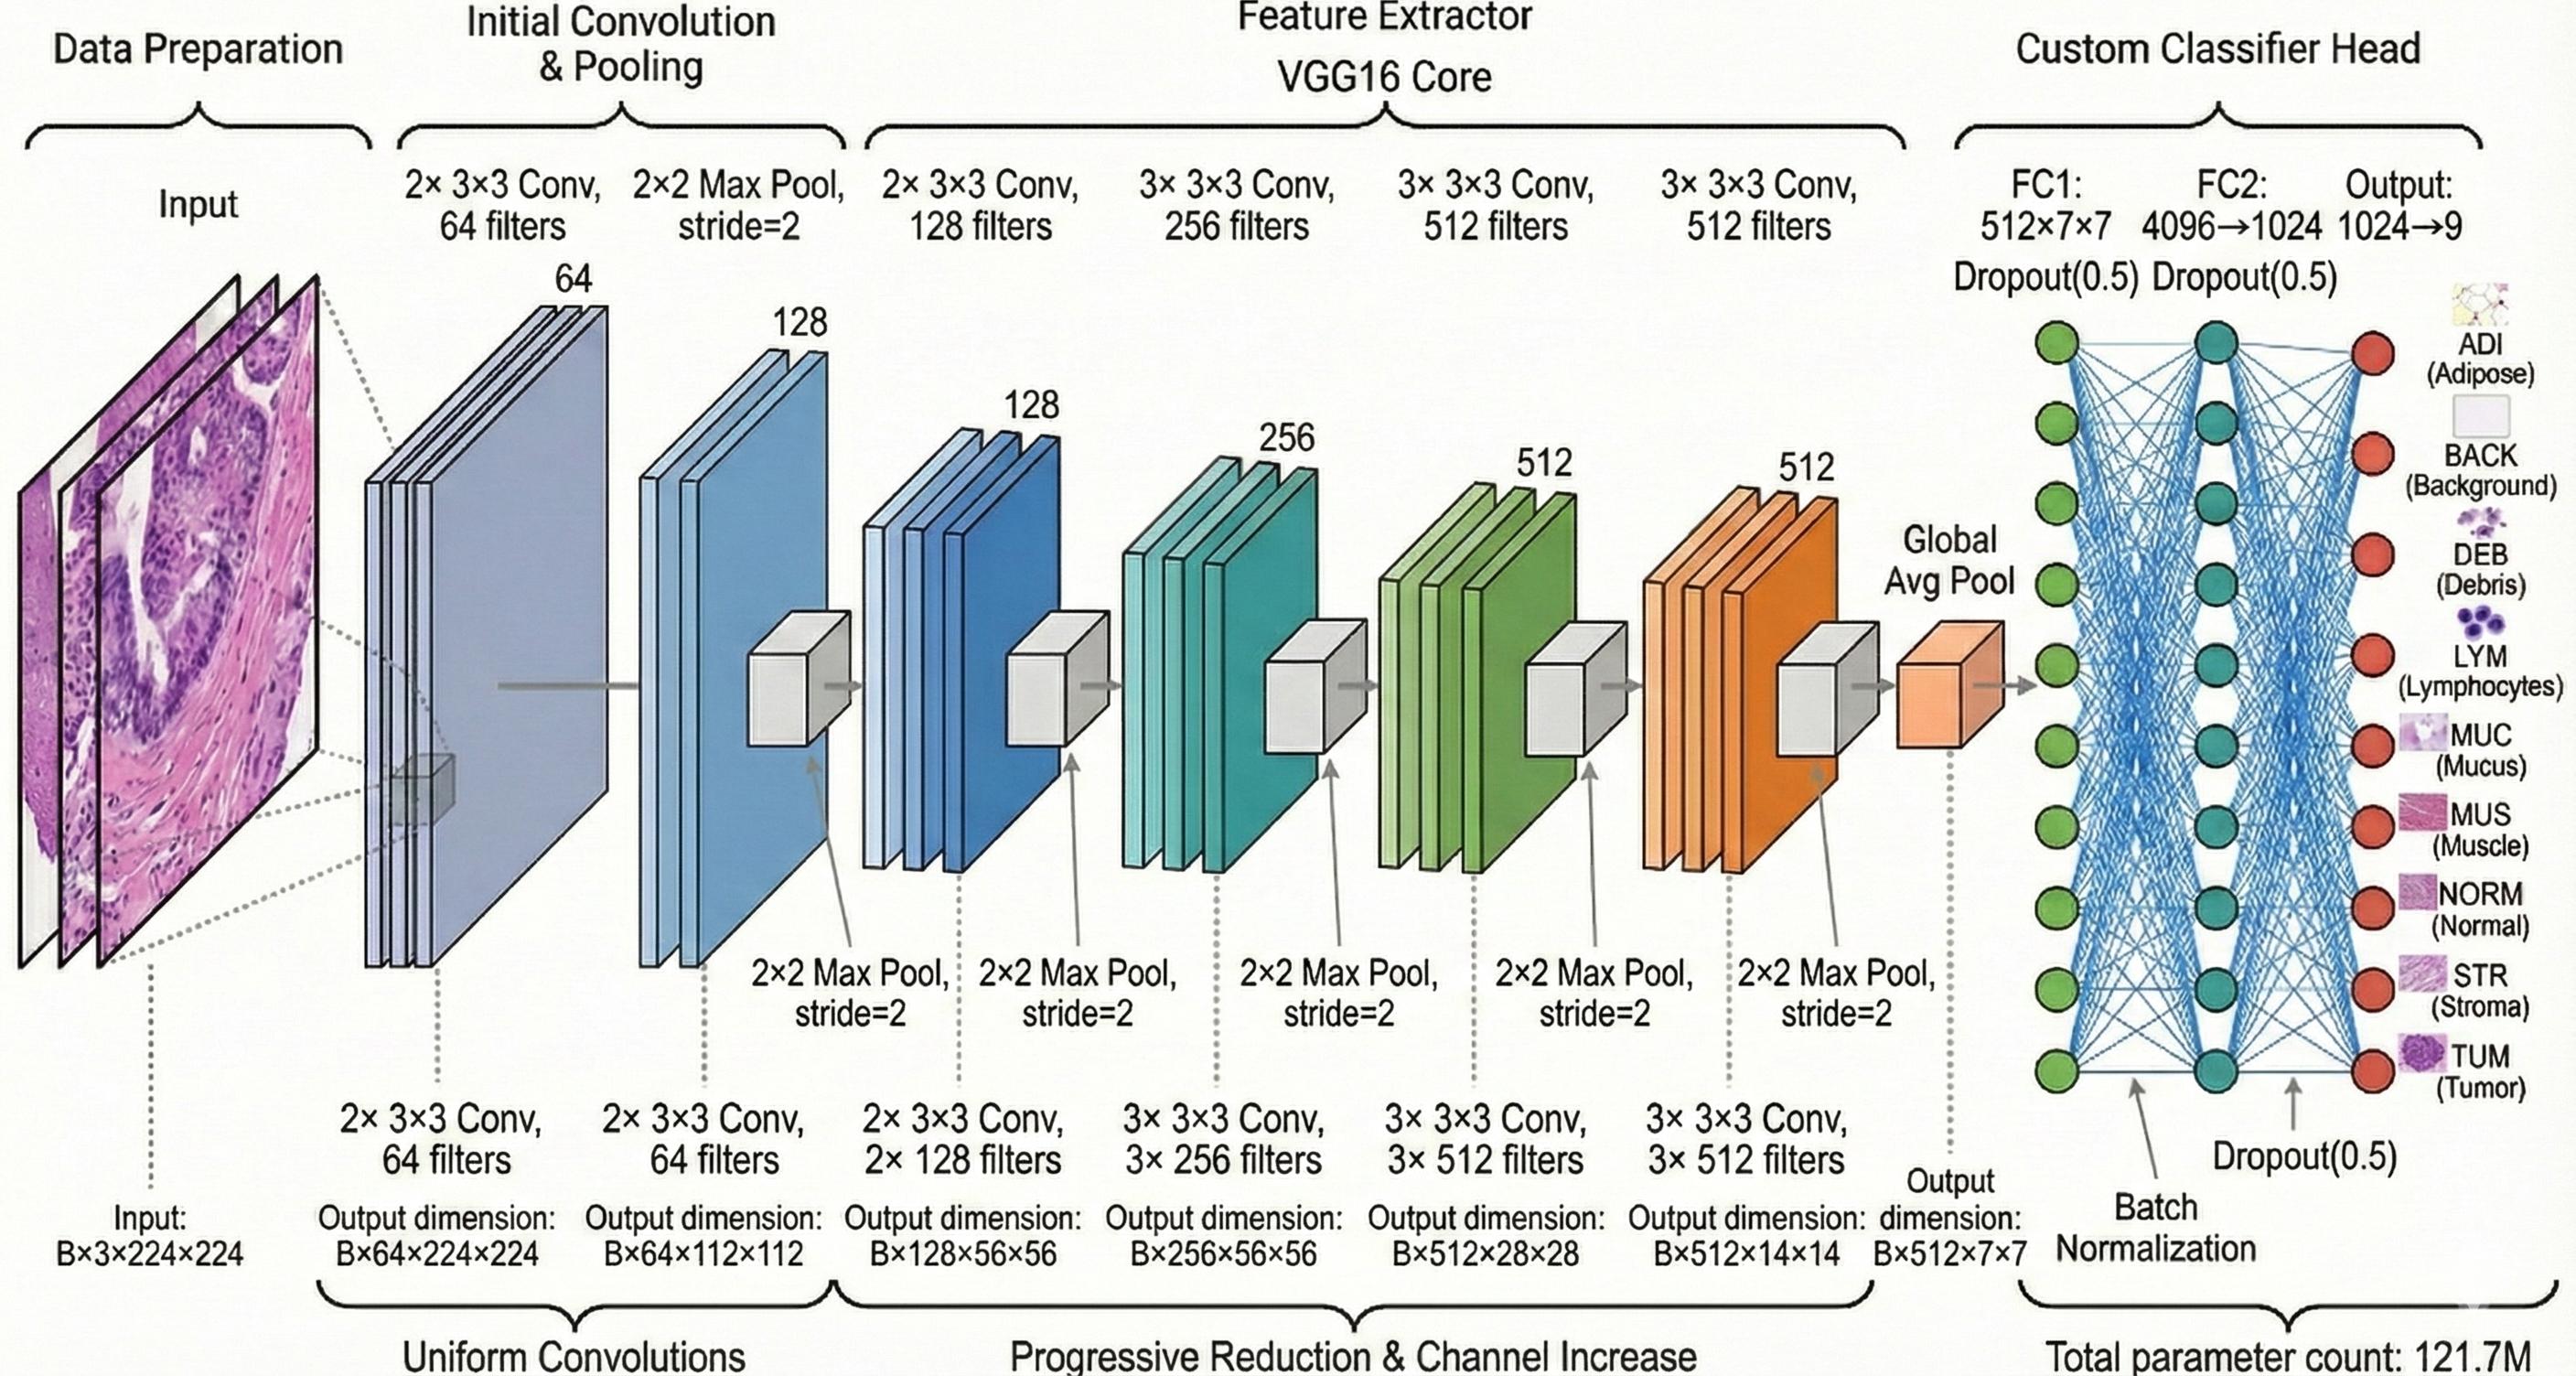
\includegraphics[width=.8\linewidth]{../vgg16/ARCH.png}
%     \caption{VGG-16 architecture diagram showing the sequential convolutional blocks and custom classifier head adapted for 9-class histopathology tissue classification.}
%     \label{fig.vgg16_arch}
% \end{figure}

\subsubsection{ResNet-50 Classifier Model}
The ResNet-50 classifier adapts a residual network architecture to histopathology image analysis via transfer learning. Individual images are processed through ResNet-50, initialized with pretrained weights, with the final fully connected layer replaced by a domain-specific classifier head. The ResNet-50 architecture employs a bottleneck design with residual connections enabling training of very deep networks. The backbone structure consists of: (1) Initial 7$\times$7 conv with 64 filters, stride=2, padding=3 $\rightarrow$ 3$\times$3 max pool with stride=2; (2) Four sequential stages with bottleneck blocks: Stage 1 (3 blocks, 256 filters), Stage 2 (4 blocks, 512 filters), Stage 3 (6 blocks, 1024 filters), Stage 4 (3 blocks, 2048 filters); followed by adaptive average pooling. The custom classifier head includes: (1) Linear(2048 $\rightarrow$ 512) + BatchNorm1D + ReLU + Dropout(0.5) with 1,049,088 parameters; (2) Linear(512 $\rightarrow$ 256) + BatchNorm1D + ReLU + Dropout(0.4) with 131,328 parameters; (3) Linear(256 $\rightarrow$ 9) with 2,313 parameters for 9-class classification. This model uses skip connections within its backbone to enable deeper feature representation, which is beneficial for capturing complex patterns in histopathological images. The total parameter count is 24.7M with a memory footprint of approximately 277MB and computational complexity of 8.18 GFLOPs for forward pass. Like VGG-16, we also train both the backbone and classifier, with different learning rates.

% \begin{figure}[H]
%     \centering
%     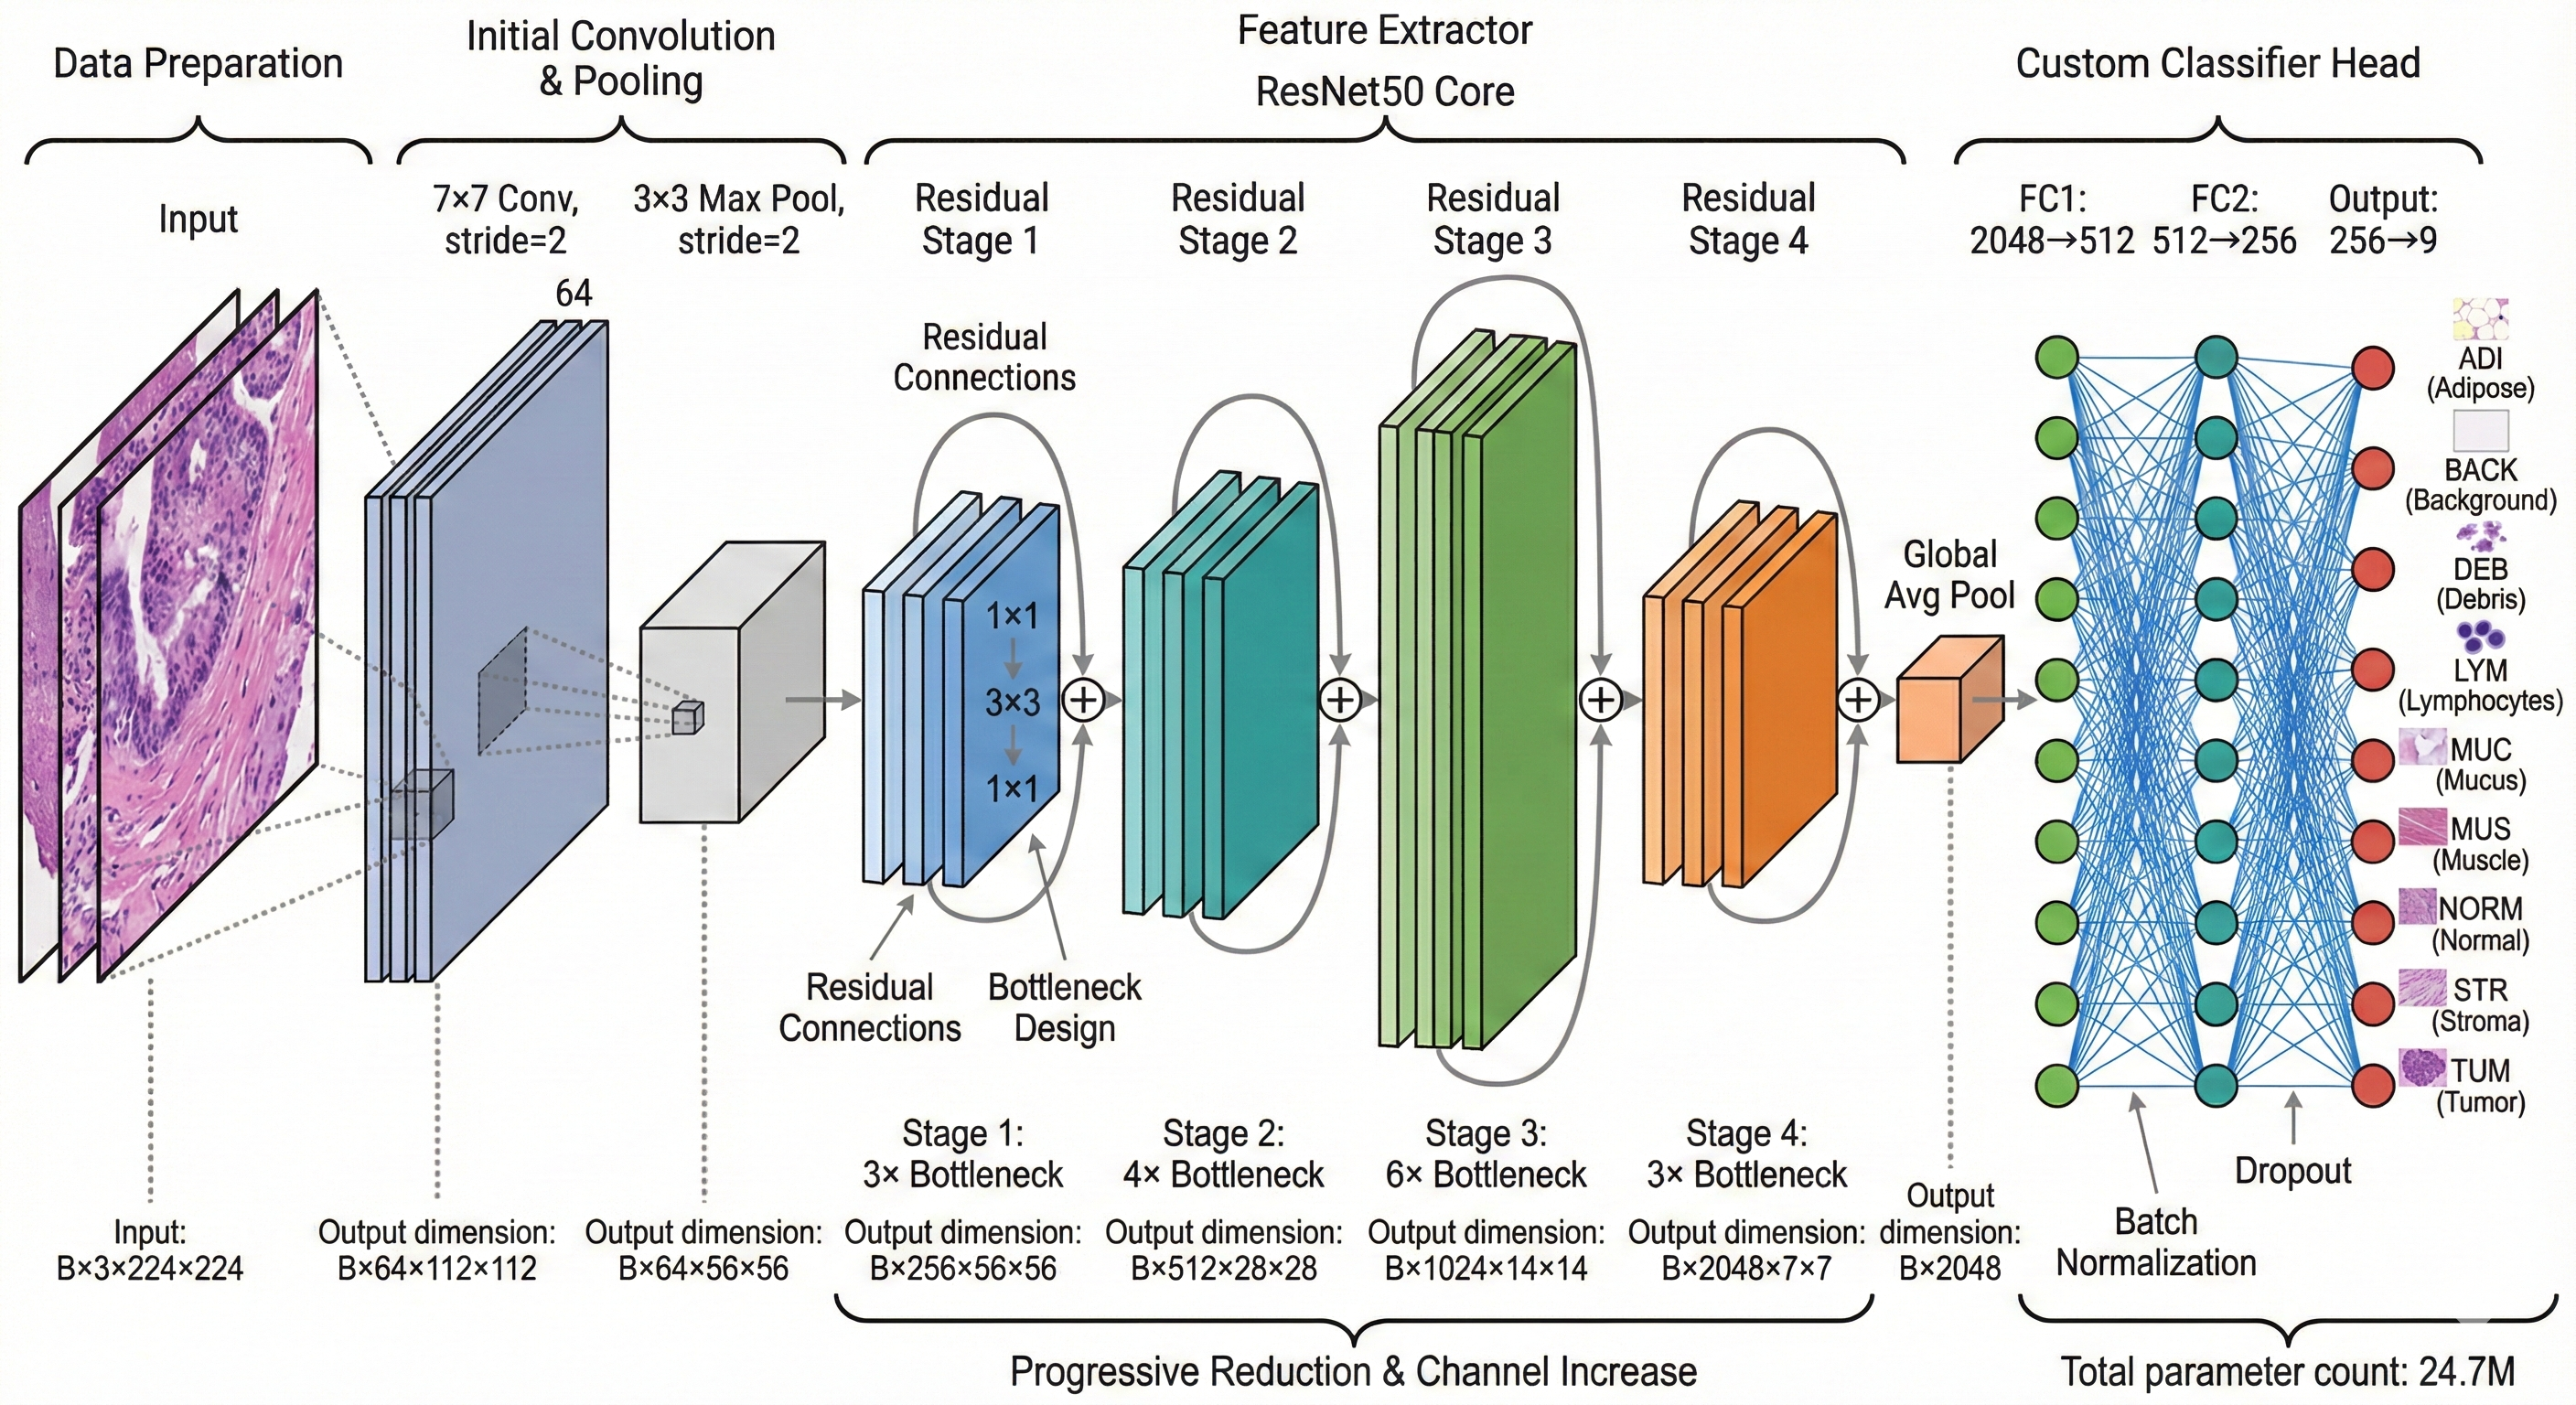
\includegraphics[width=.8\linewidth]{../resnet50/ARCH.png}
%     \caption{ResNet-50 architecture diagram illustrating the bottleneck design with residual connections and custom classifier head. Feature extracting backbone is fine-tuned from ImageNet pretrained weights for histopathology classification.}
%     \label{fig.resnet50_arch}
% \end{figure}

\subsection{Training Process}
All models were trained using a supervised learning approach with cross-entropy loss optimization. Training is executed on a NVIDIA RTX 4090, with TensorBoard logging for loss tracking. Early stopping is implemented to prevent overfitting by monitoring validation metrics with configurable patience and minimum delta thresholds.

Training time analysis reveals significant efficiency advantages for ViT-based approaches when considering total development time (Figure~\ref{fig.train_comp}). Traditional CNN architectures required substantially longer training: ResNet-50 (24.7 M params) converged in 61 minutes, while VGG-16 (121.7 M params) needed 79 minutes due to its larger parameter count.

For ViT-based methods, we cache the Virchow2 embeddings to avoid end-to-end training, which significantly reduces computational requirements. We include the 9.5-minute embedding preprocessing time as a necessary one-time step. PatchMIL (0.86 M params) required 8.3 minutes for model training, totaling 17.8 minutes including embedding preprocessing. MulticlassMLP (0.82 M params) trained in 16.7 minutes, totaling 26.2 minutes with preprocessing.

Thus, the complete pipeline times are: VGG-16 (79 min, 121.7 M params) > ResNet-50 (61 min, 24.7 M params) > MulticlassMLP (26.2 min, 0.82 M params) > PatchMIL (17.8 min, 0.86 M params), demonstrating that foundation model-based approaches offer faster overall development, largely due to foundational model's pretrained knowledge.

\begin{figure}[H]
    \centering
    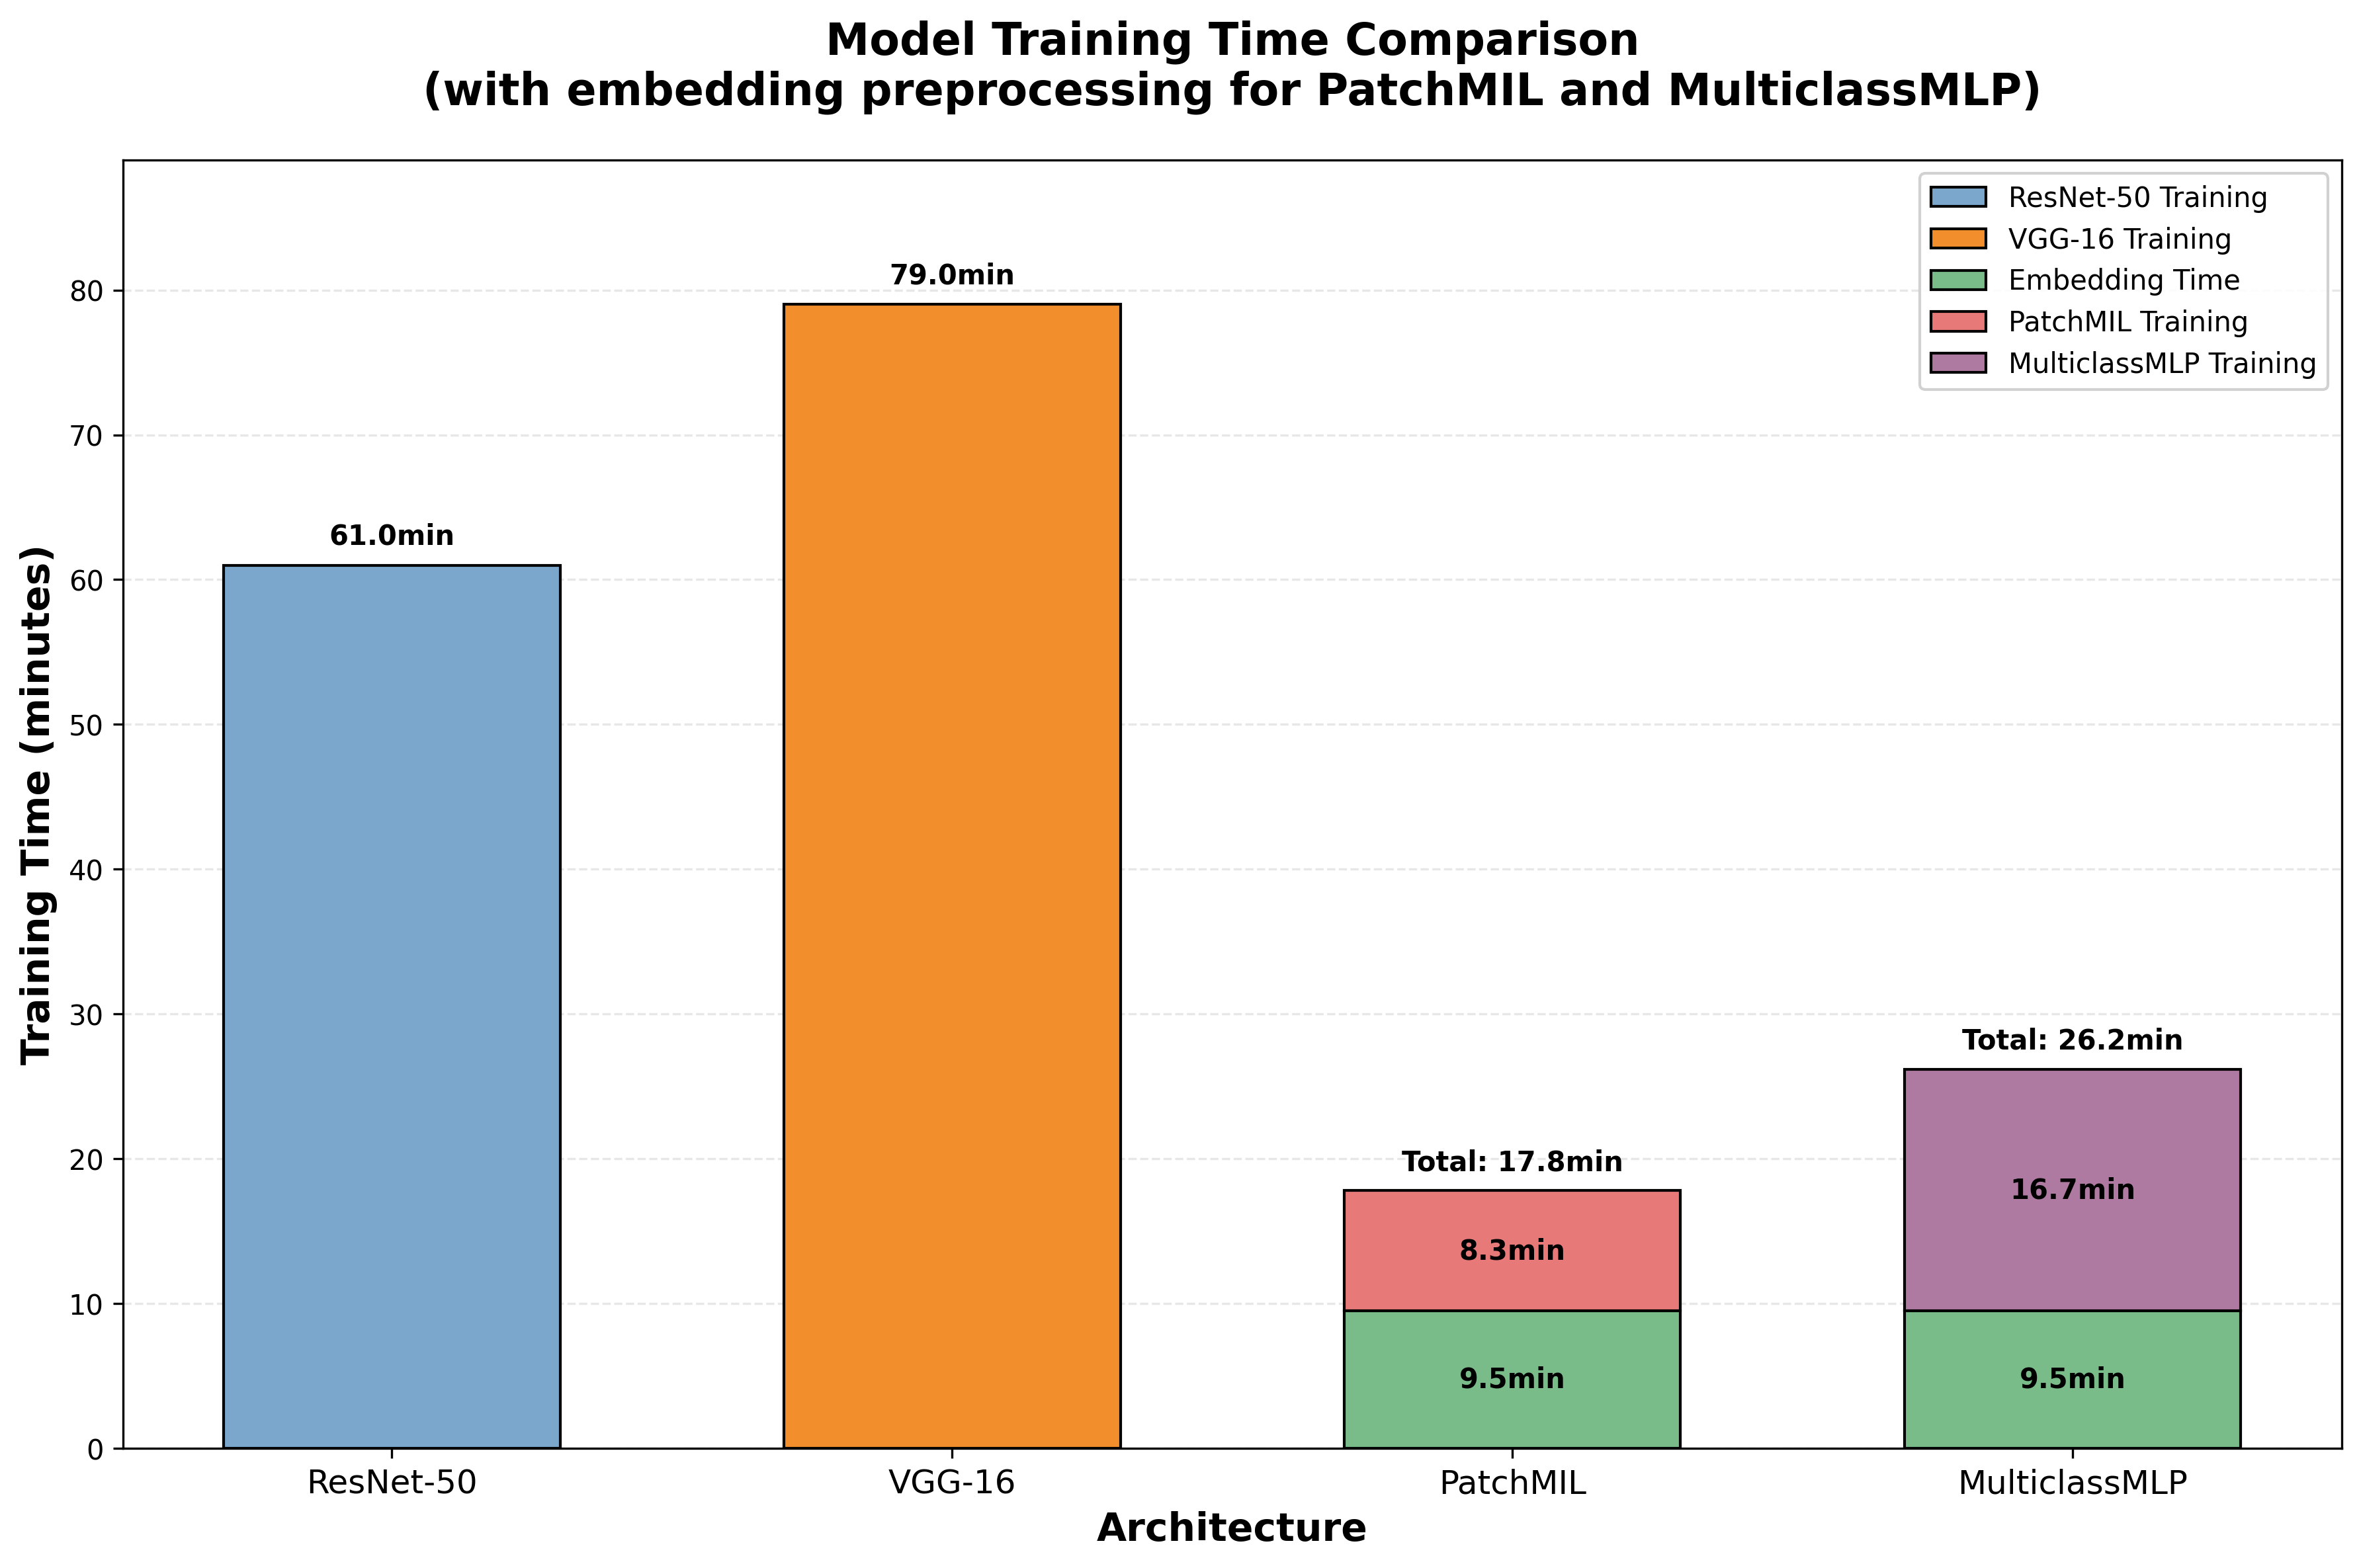
\includegraphics[width=.8\linewidth]{../training_time_comparison.png}
    \caption{Training time comparison between the different architectures.}
    \label{fig.train_comp}
\end{figure}


\section{Results}
\subsection{ViT-Based Models}
Both ViT-based models achieved near-perfect classification performance on the NCT-CRC-HE-100K dataset.
The PatchMIL model reached an overall accuracy of 0.9963, precision of 0.9965, recall of 0.9960, and F1 score of 0.9963.

\begin{figure}[H]
    \centering
    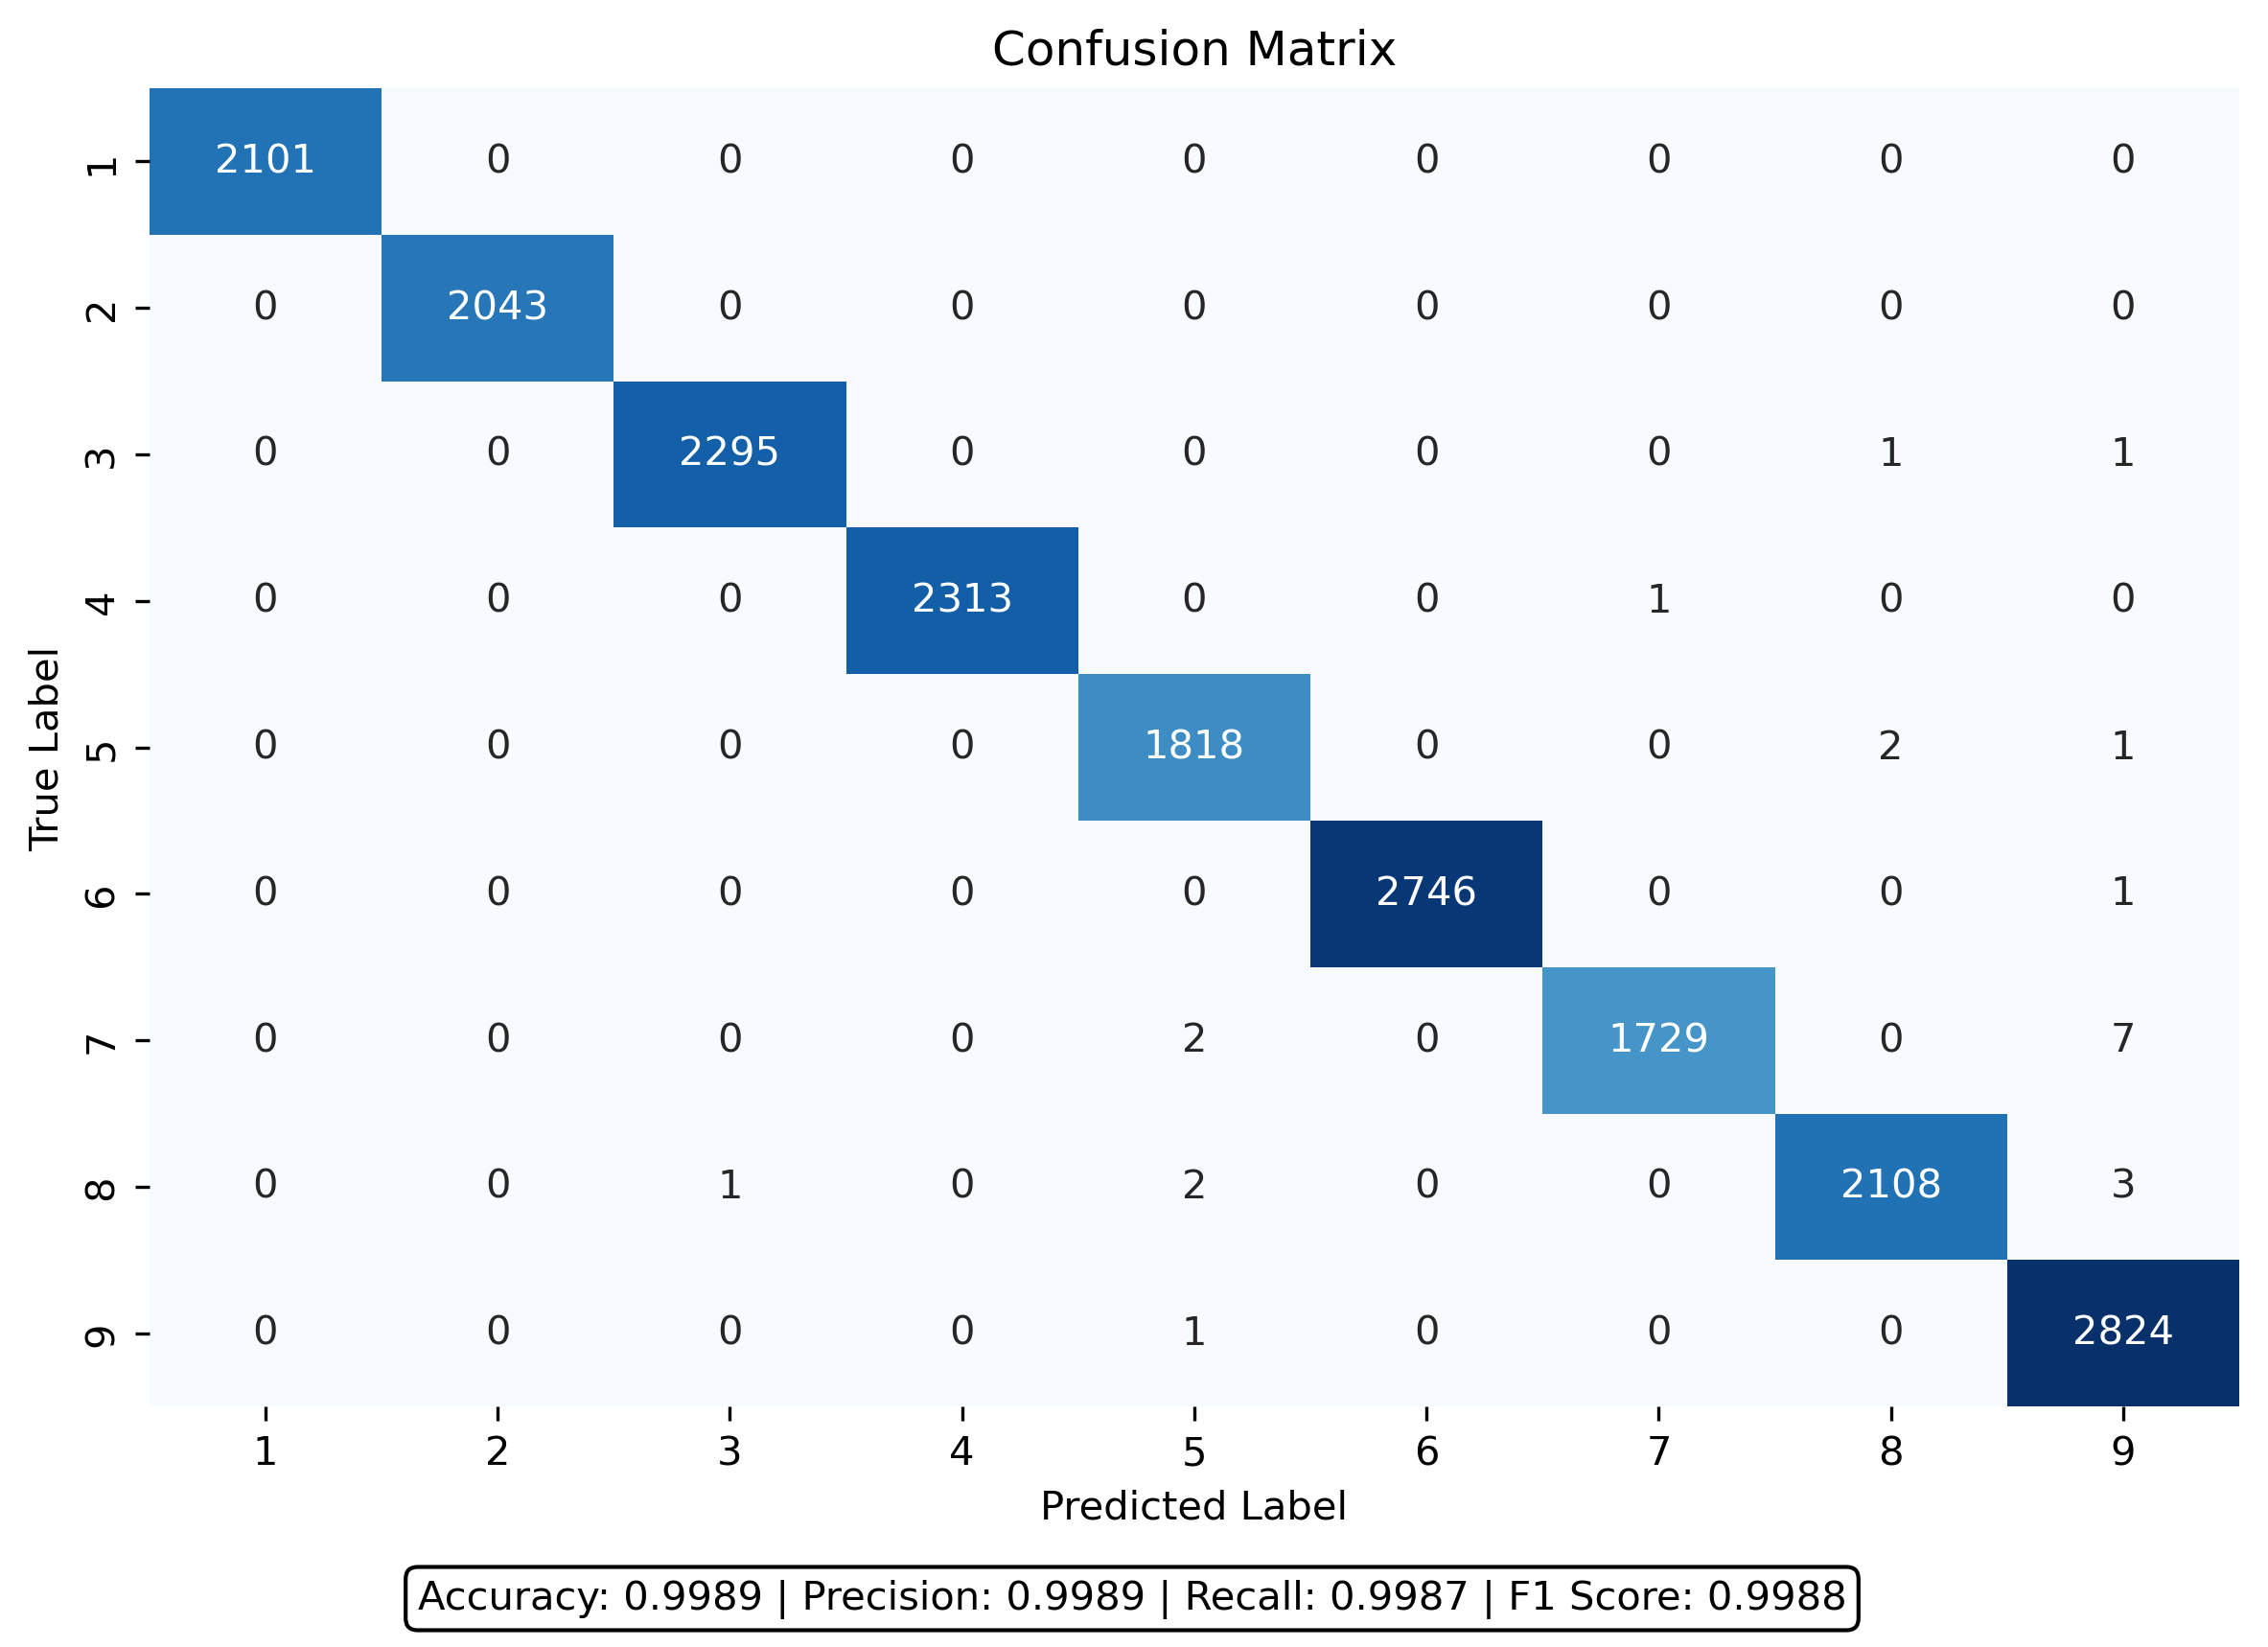
\includegraphics[width=.8\linewidth]{../runs/v1.0_cls/figs/confusion_matrix.png}
    \caption{Confusion matrix for MulticlassMLP classification.}
    \label{fig.conf_mat_cls}
\end{figure}

The MulticlassMLP model slightly surpassed it with accuracy, precision, recall, and F1 score all equal to 0.9983.

\begin{figure}[H]
    \centering
    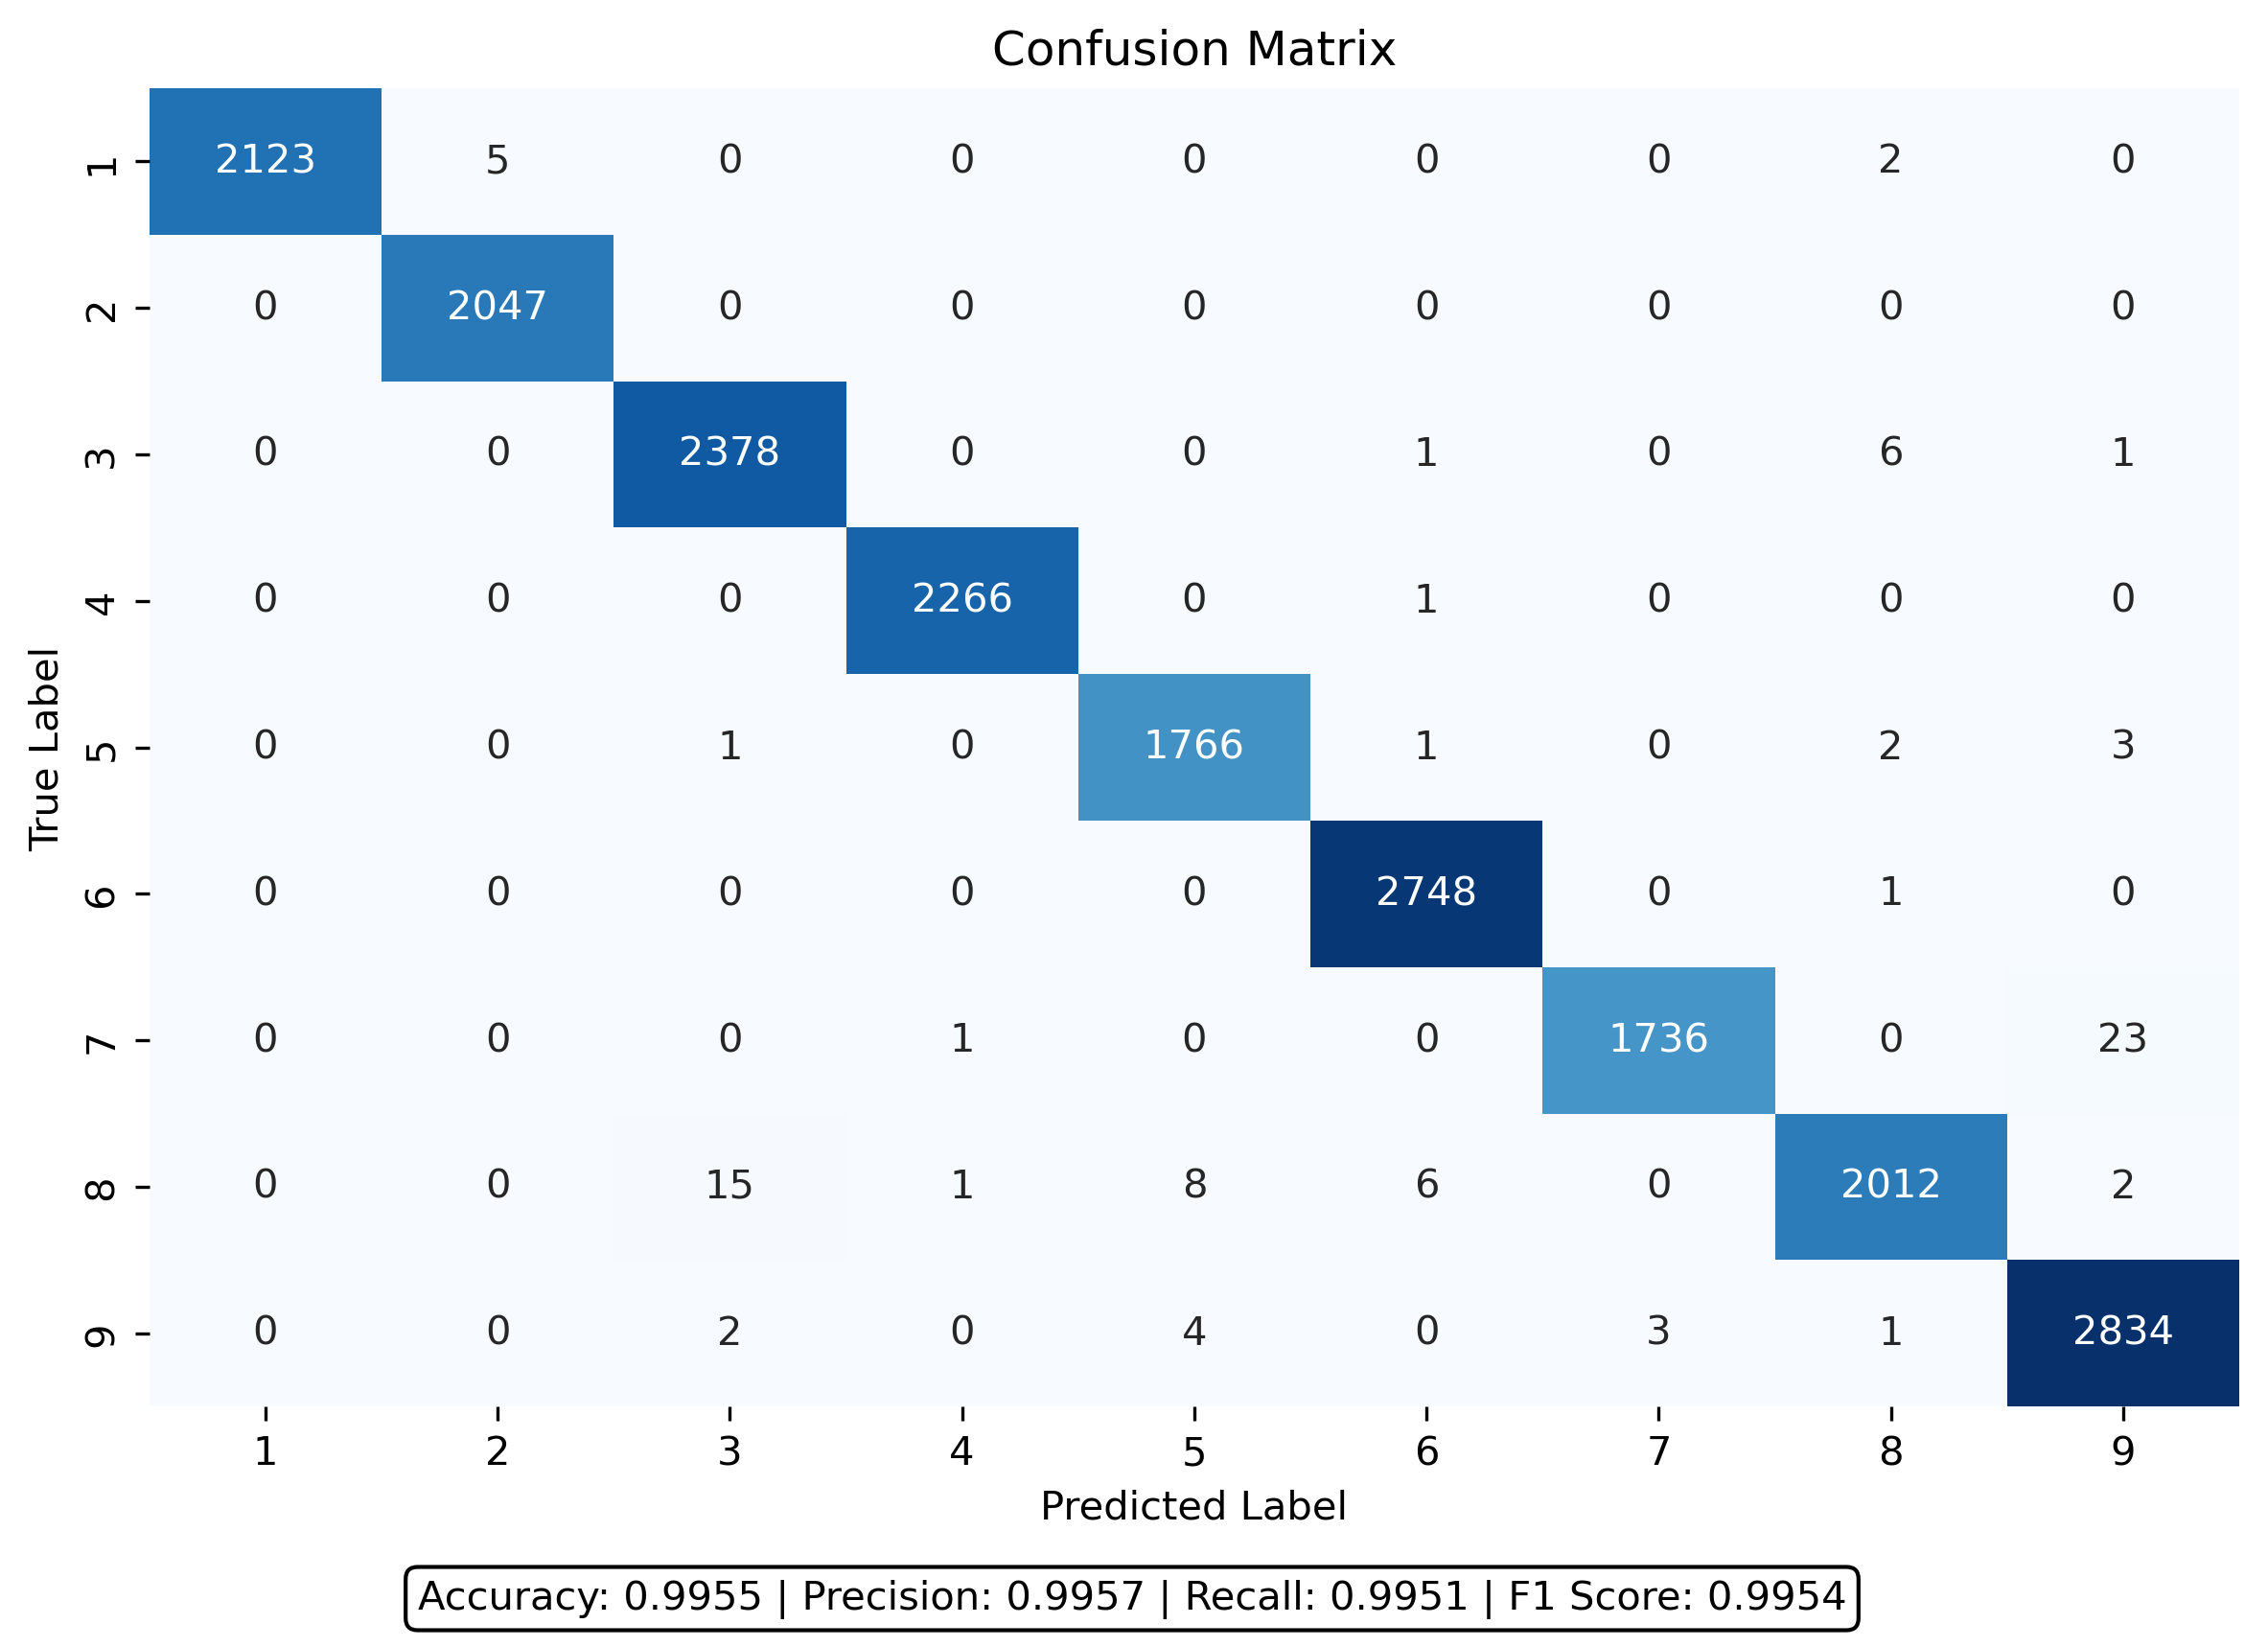
\includegraphics[width=.8\linewidth]{../runs/v1.0_patch/figs/confusion_matrix.png}
    \caption{Confusion matrix for PatchMIL classification.}
    \label{fig.conf_mat_patch}
\end{figure}

For both models, the macro-average ROC-AUC was 1.00, and each individual tissue class (ADI, BACK, DEB, LYM, MUC, MUS, NORM, STR, TUM) achieved an AUC of 1.00, indicating excellent separability across all histological subtypes.

\begin{figure}[H]
    \centering
    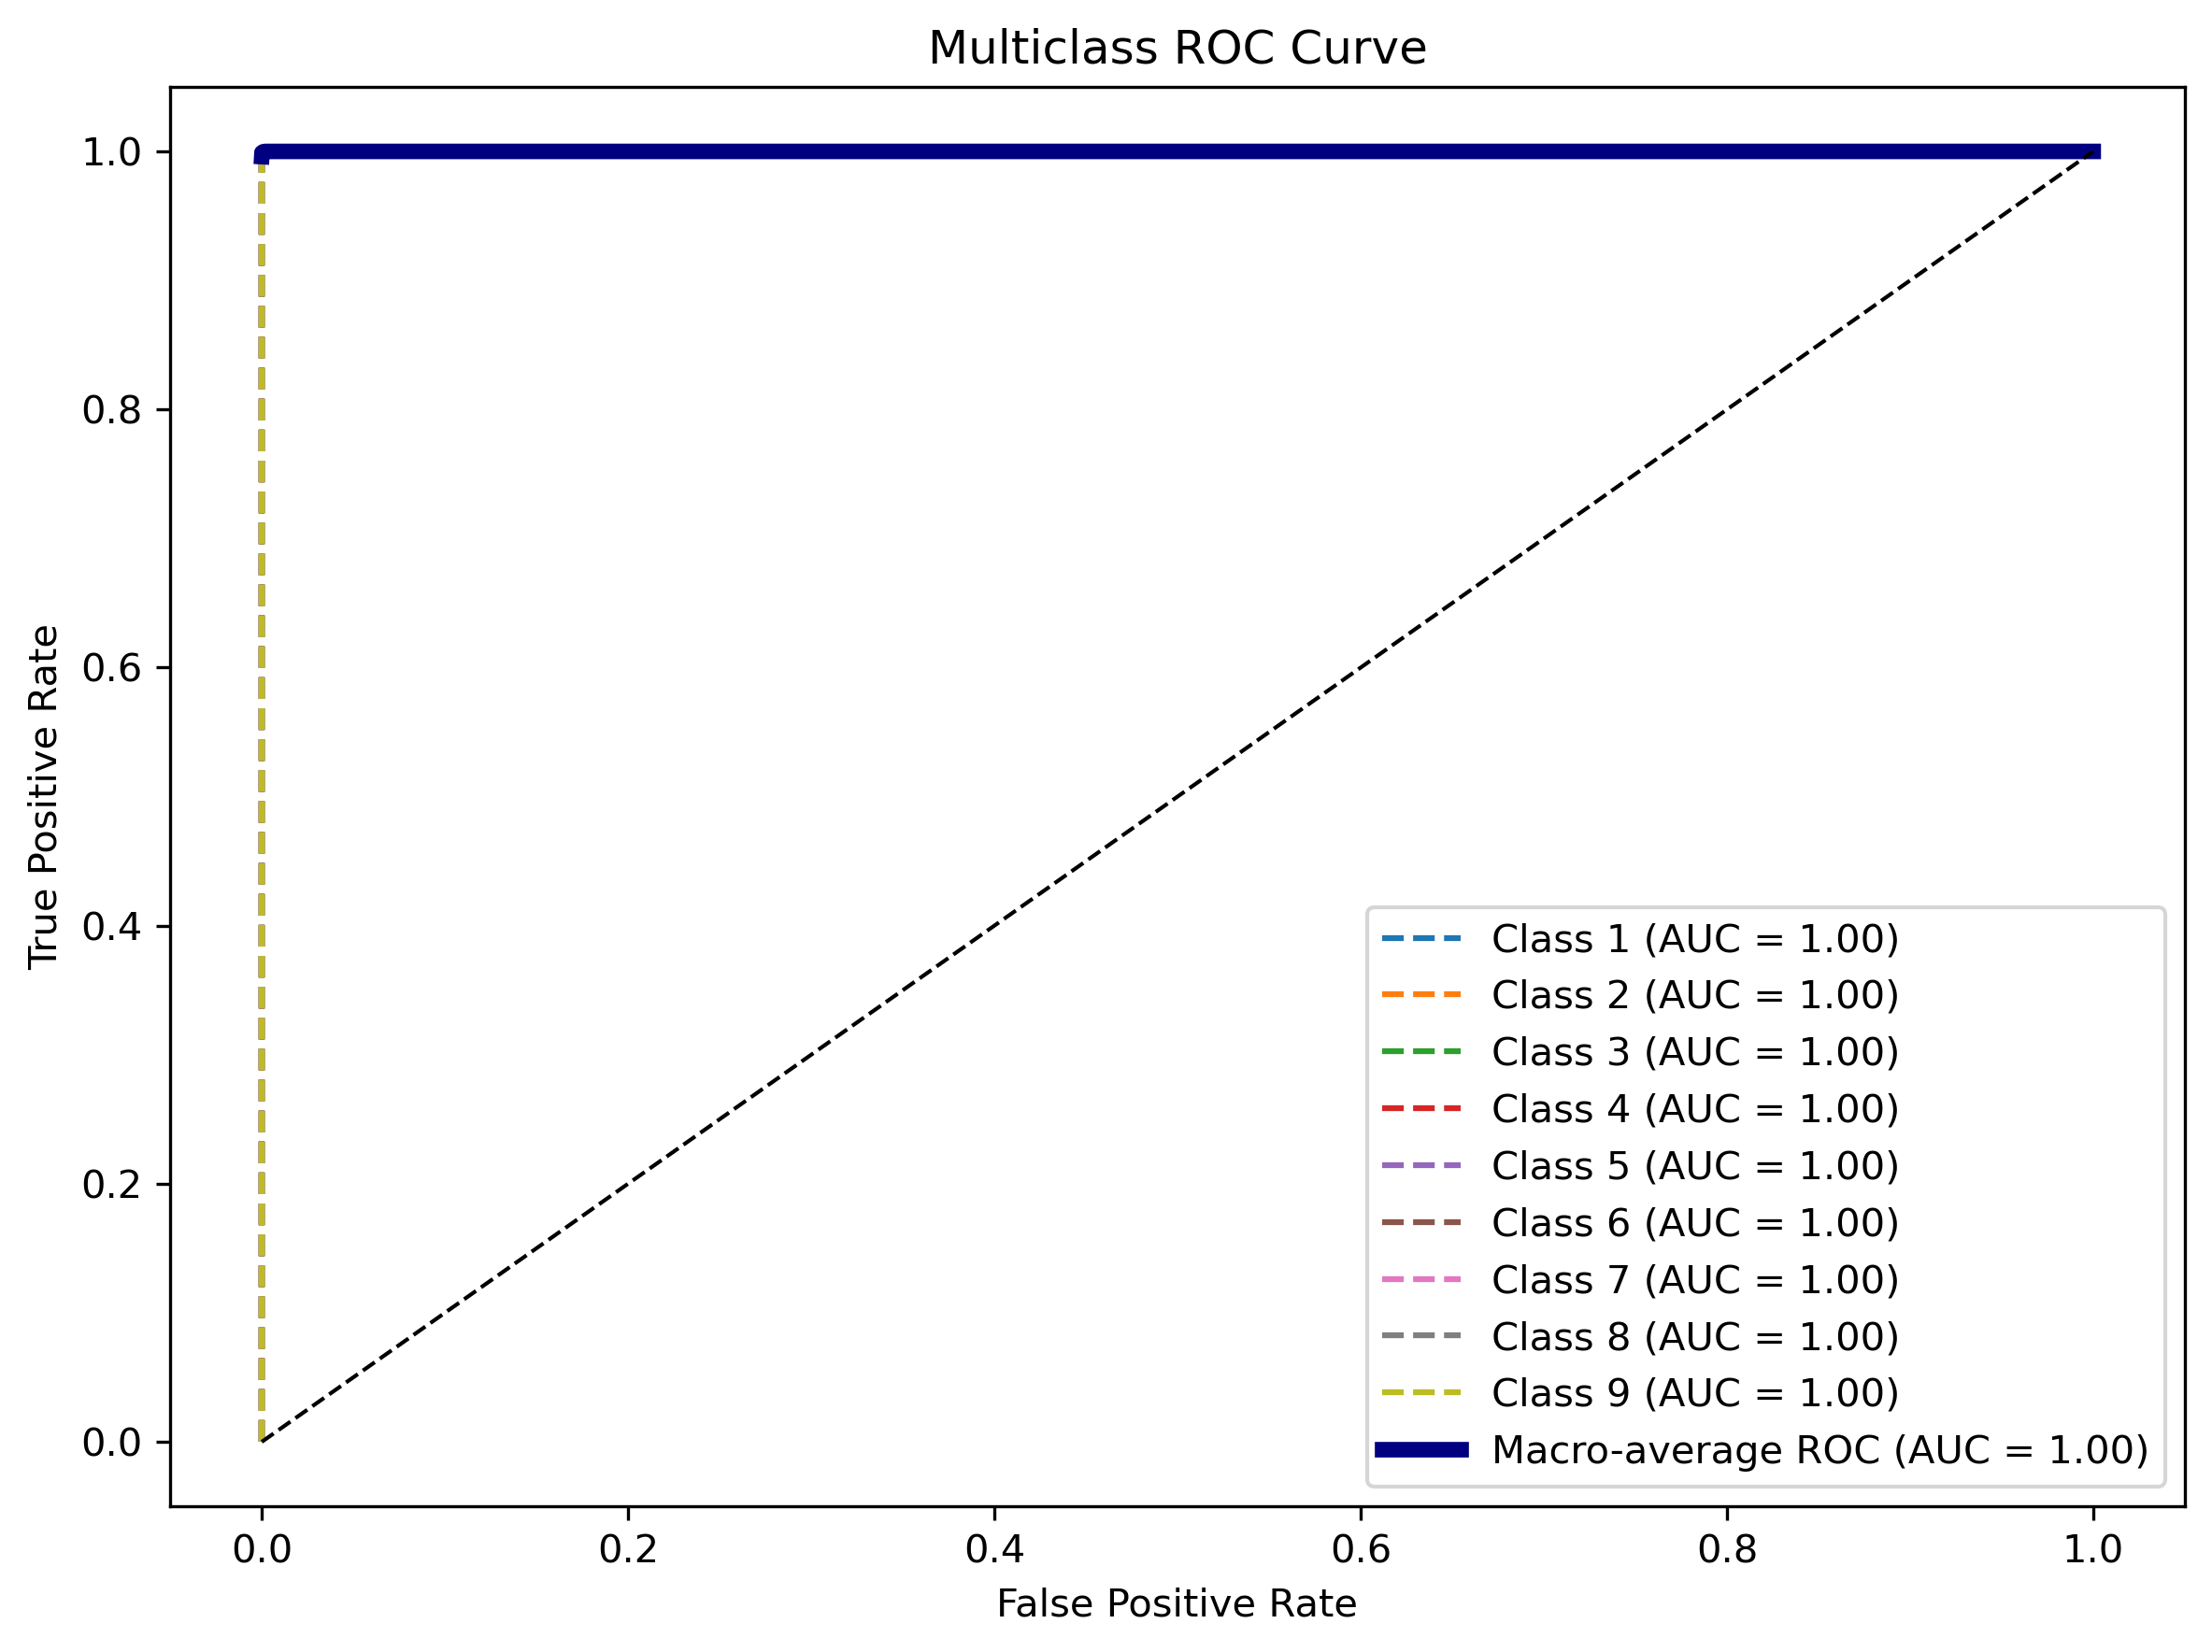
\includegraphics[width=.8\linewidth]{../runs/v1.0_cls/figs/ROC_curve.png}
    \caption{Multiclass receiver operating characteristic (ROC) curve for MulticlassMLP classification.}
    \label{fig.roc_cls}
\end{figure}

\begin{figure}[H]
    \centering
    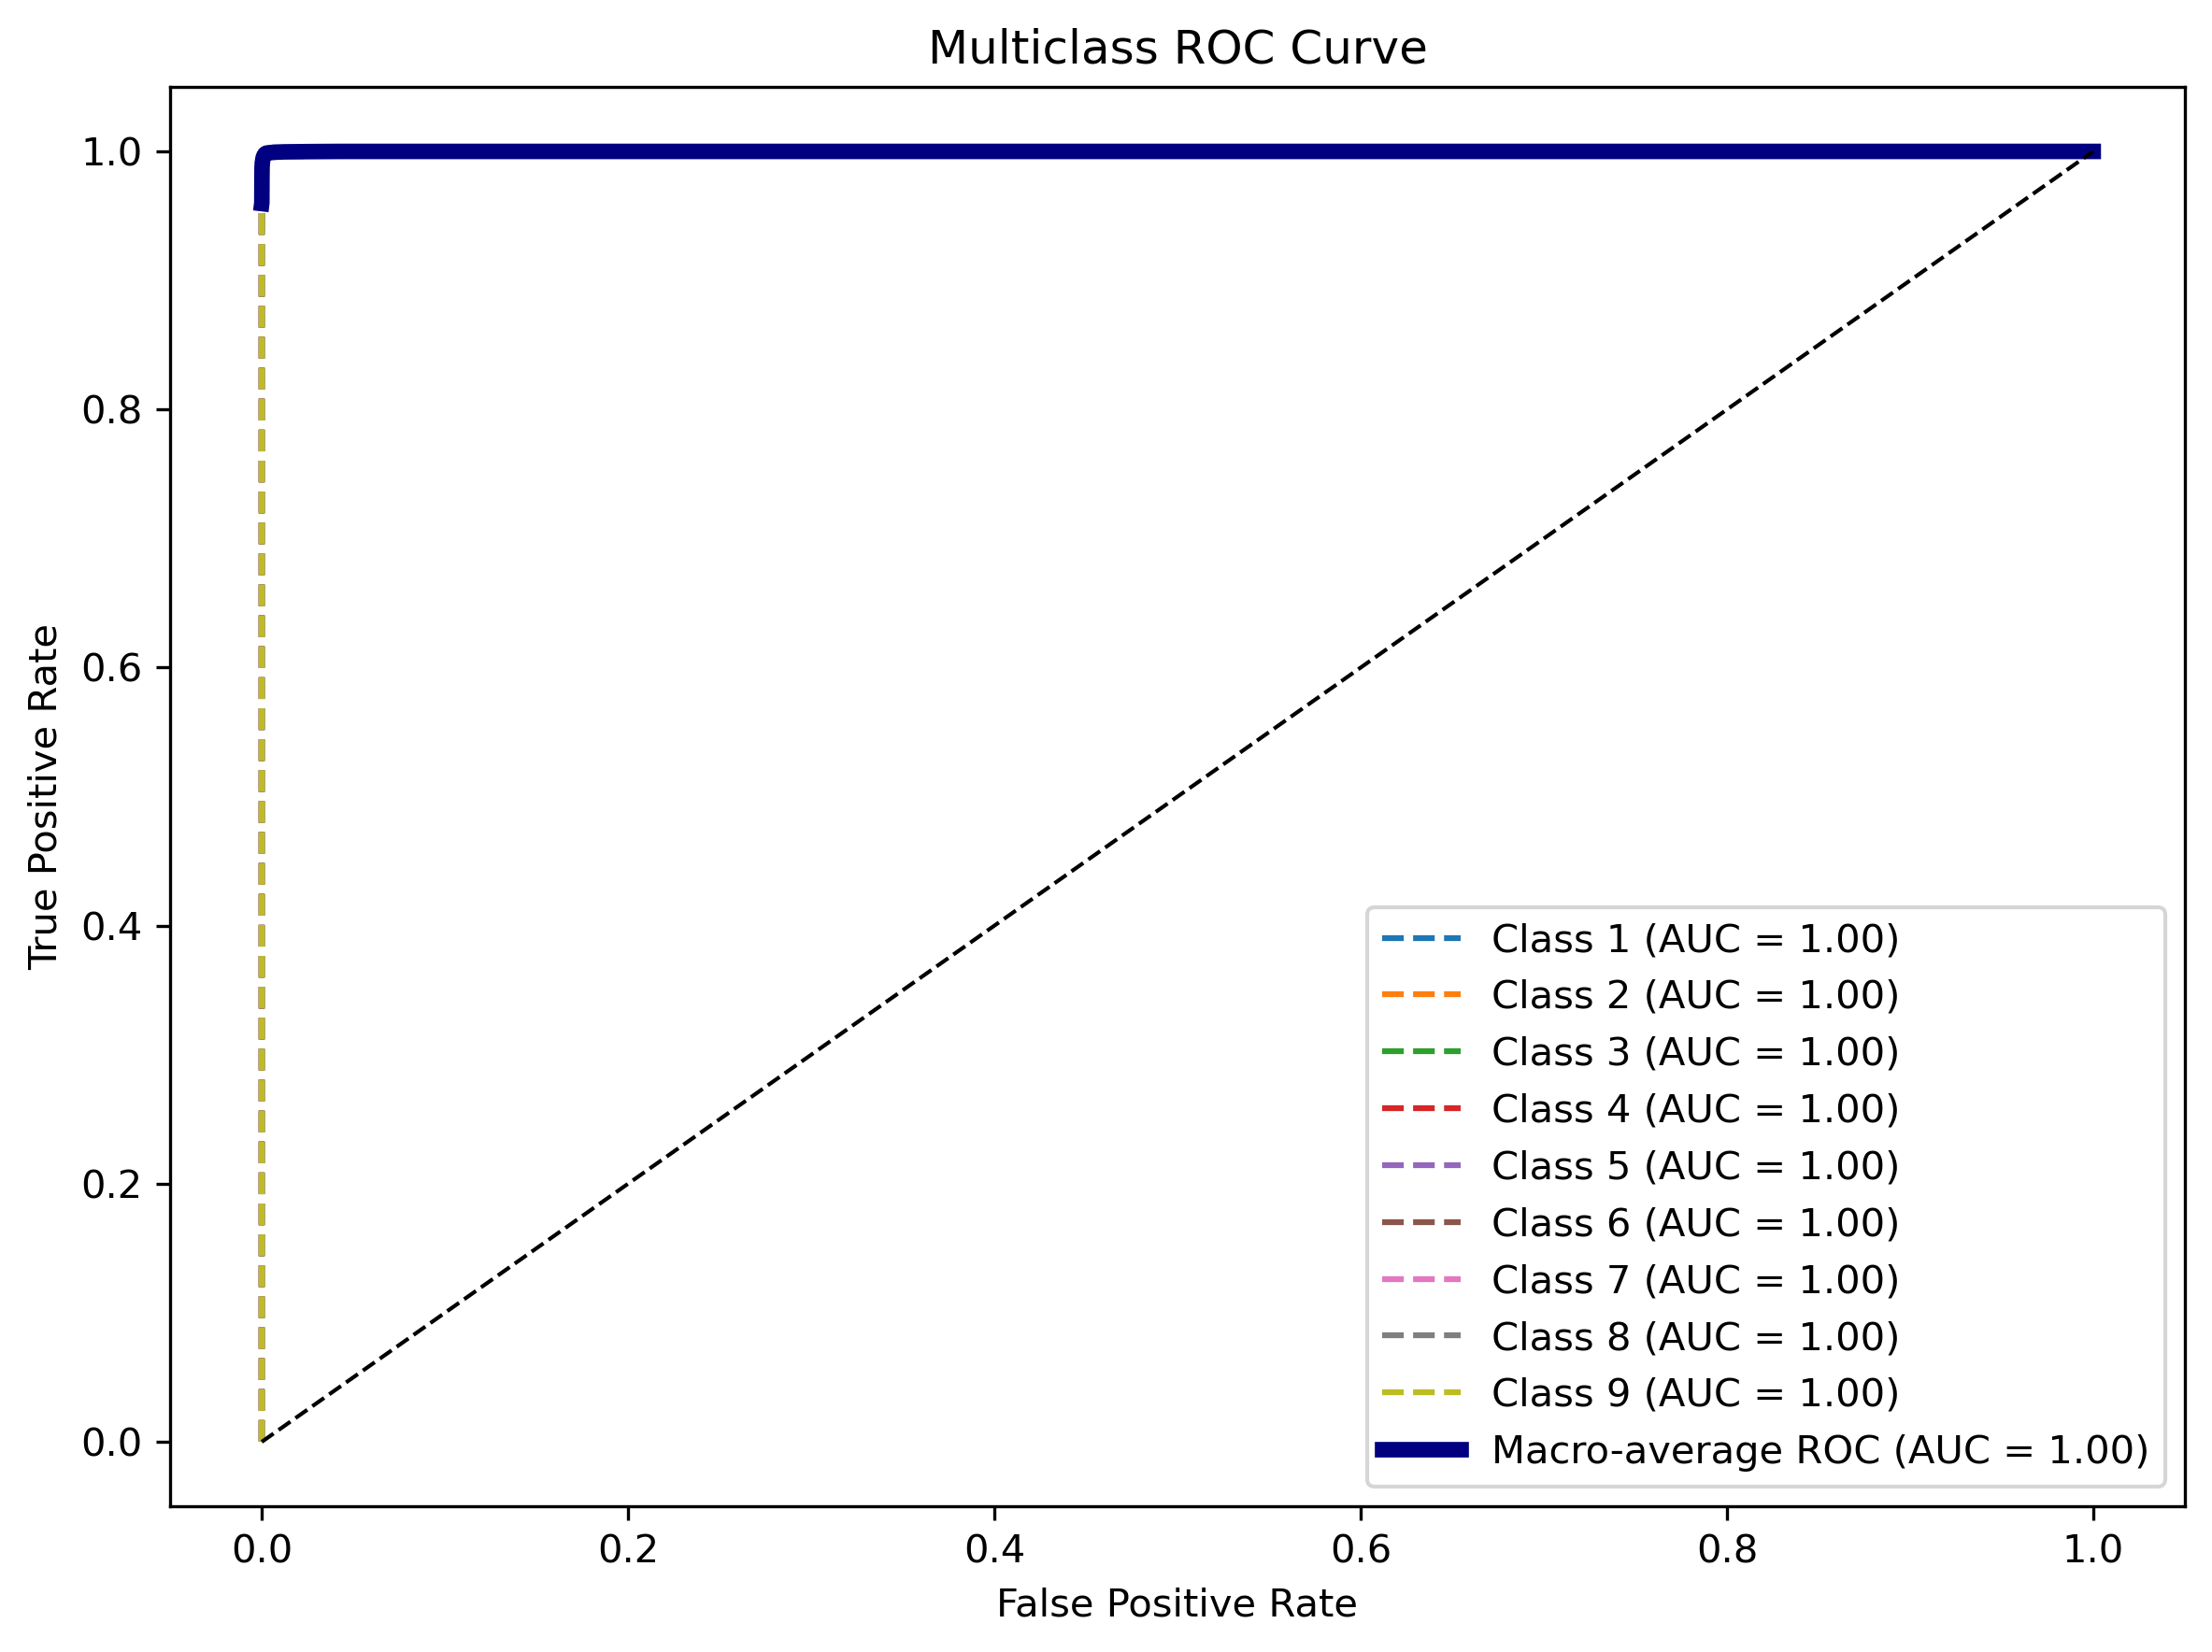
\includegraphics[width=.8\linewidth]{../runs/v1.0_patch/figs/ROC_curve.png}
    \caption{Multiclass receiver operating characteristic (ROC) curve for PatchMIL classification.}
    \label{fig.roc_patch}
\end{figure}

The confusion matrices show strong diagonal dominance, confirming stable discrimination among all nine tissue classes.

For PatchMIL, a few misclassifications occurred between morphologically similar categories such as stroma (STR) and tumor epithelium (TUM), or mucus (MUC) and tumor, as well as rare overlaps between debris (DEB) and adjacent tissue types. In contrast, the MulticlassMLP produced an even cleaner matrix, with only a handful of MUC $\rightarrow$ TUM and STR $\rightarrow$ TUM errors. These patterns are consistent with histopathological reality, as tumor-adjacent stroma and mucus regions often share overlapping color, texture, and glandular structures under H\&E staining.

From a computational standpoint, both models converged within 15-18 epochs under early stopping. PatchMIL required greater GPU memory and computation due to processing 256 patch tokens with an attention mechanism, whereas the CLS token based MLP operated much faster and more efficiently by using only the global embedding from the ViT feature extractor.

Overall, both ViT-based models demonstrated exceptional accuracy and robustness, with the MLP excelling in efficiency and PatchMIL offering richer interpretability through its attention weights.

\subsection{CNN-Based Models}
For CNN-based models, we also observed that both ResNet-50 and VGG-16 achieved strong performance on the NCT-CRC-HE-100K test set (Figures \ref{fig.conf_mat_resnet}-\ref{fig.roc_vgg}). ResNet-50 obtained an overall accuracy of 0.9960, with macro precision 0.9958, recall 0.9961, and F1 score 0.9959. VGG-16 performed slightly worse but still competitively, reaching an accuracy of 0.9849, precision 0.9861, recall 0.9838, and F1 score 0.9849. For both CNN architectures, the macro-average ROC–AUC was 1.00, and each of the nine tissue classes achieved an AUC of 1.00, indicating excellent separability at the decision threshold level.

\begin{figure}[H]
    \centering
    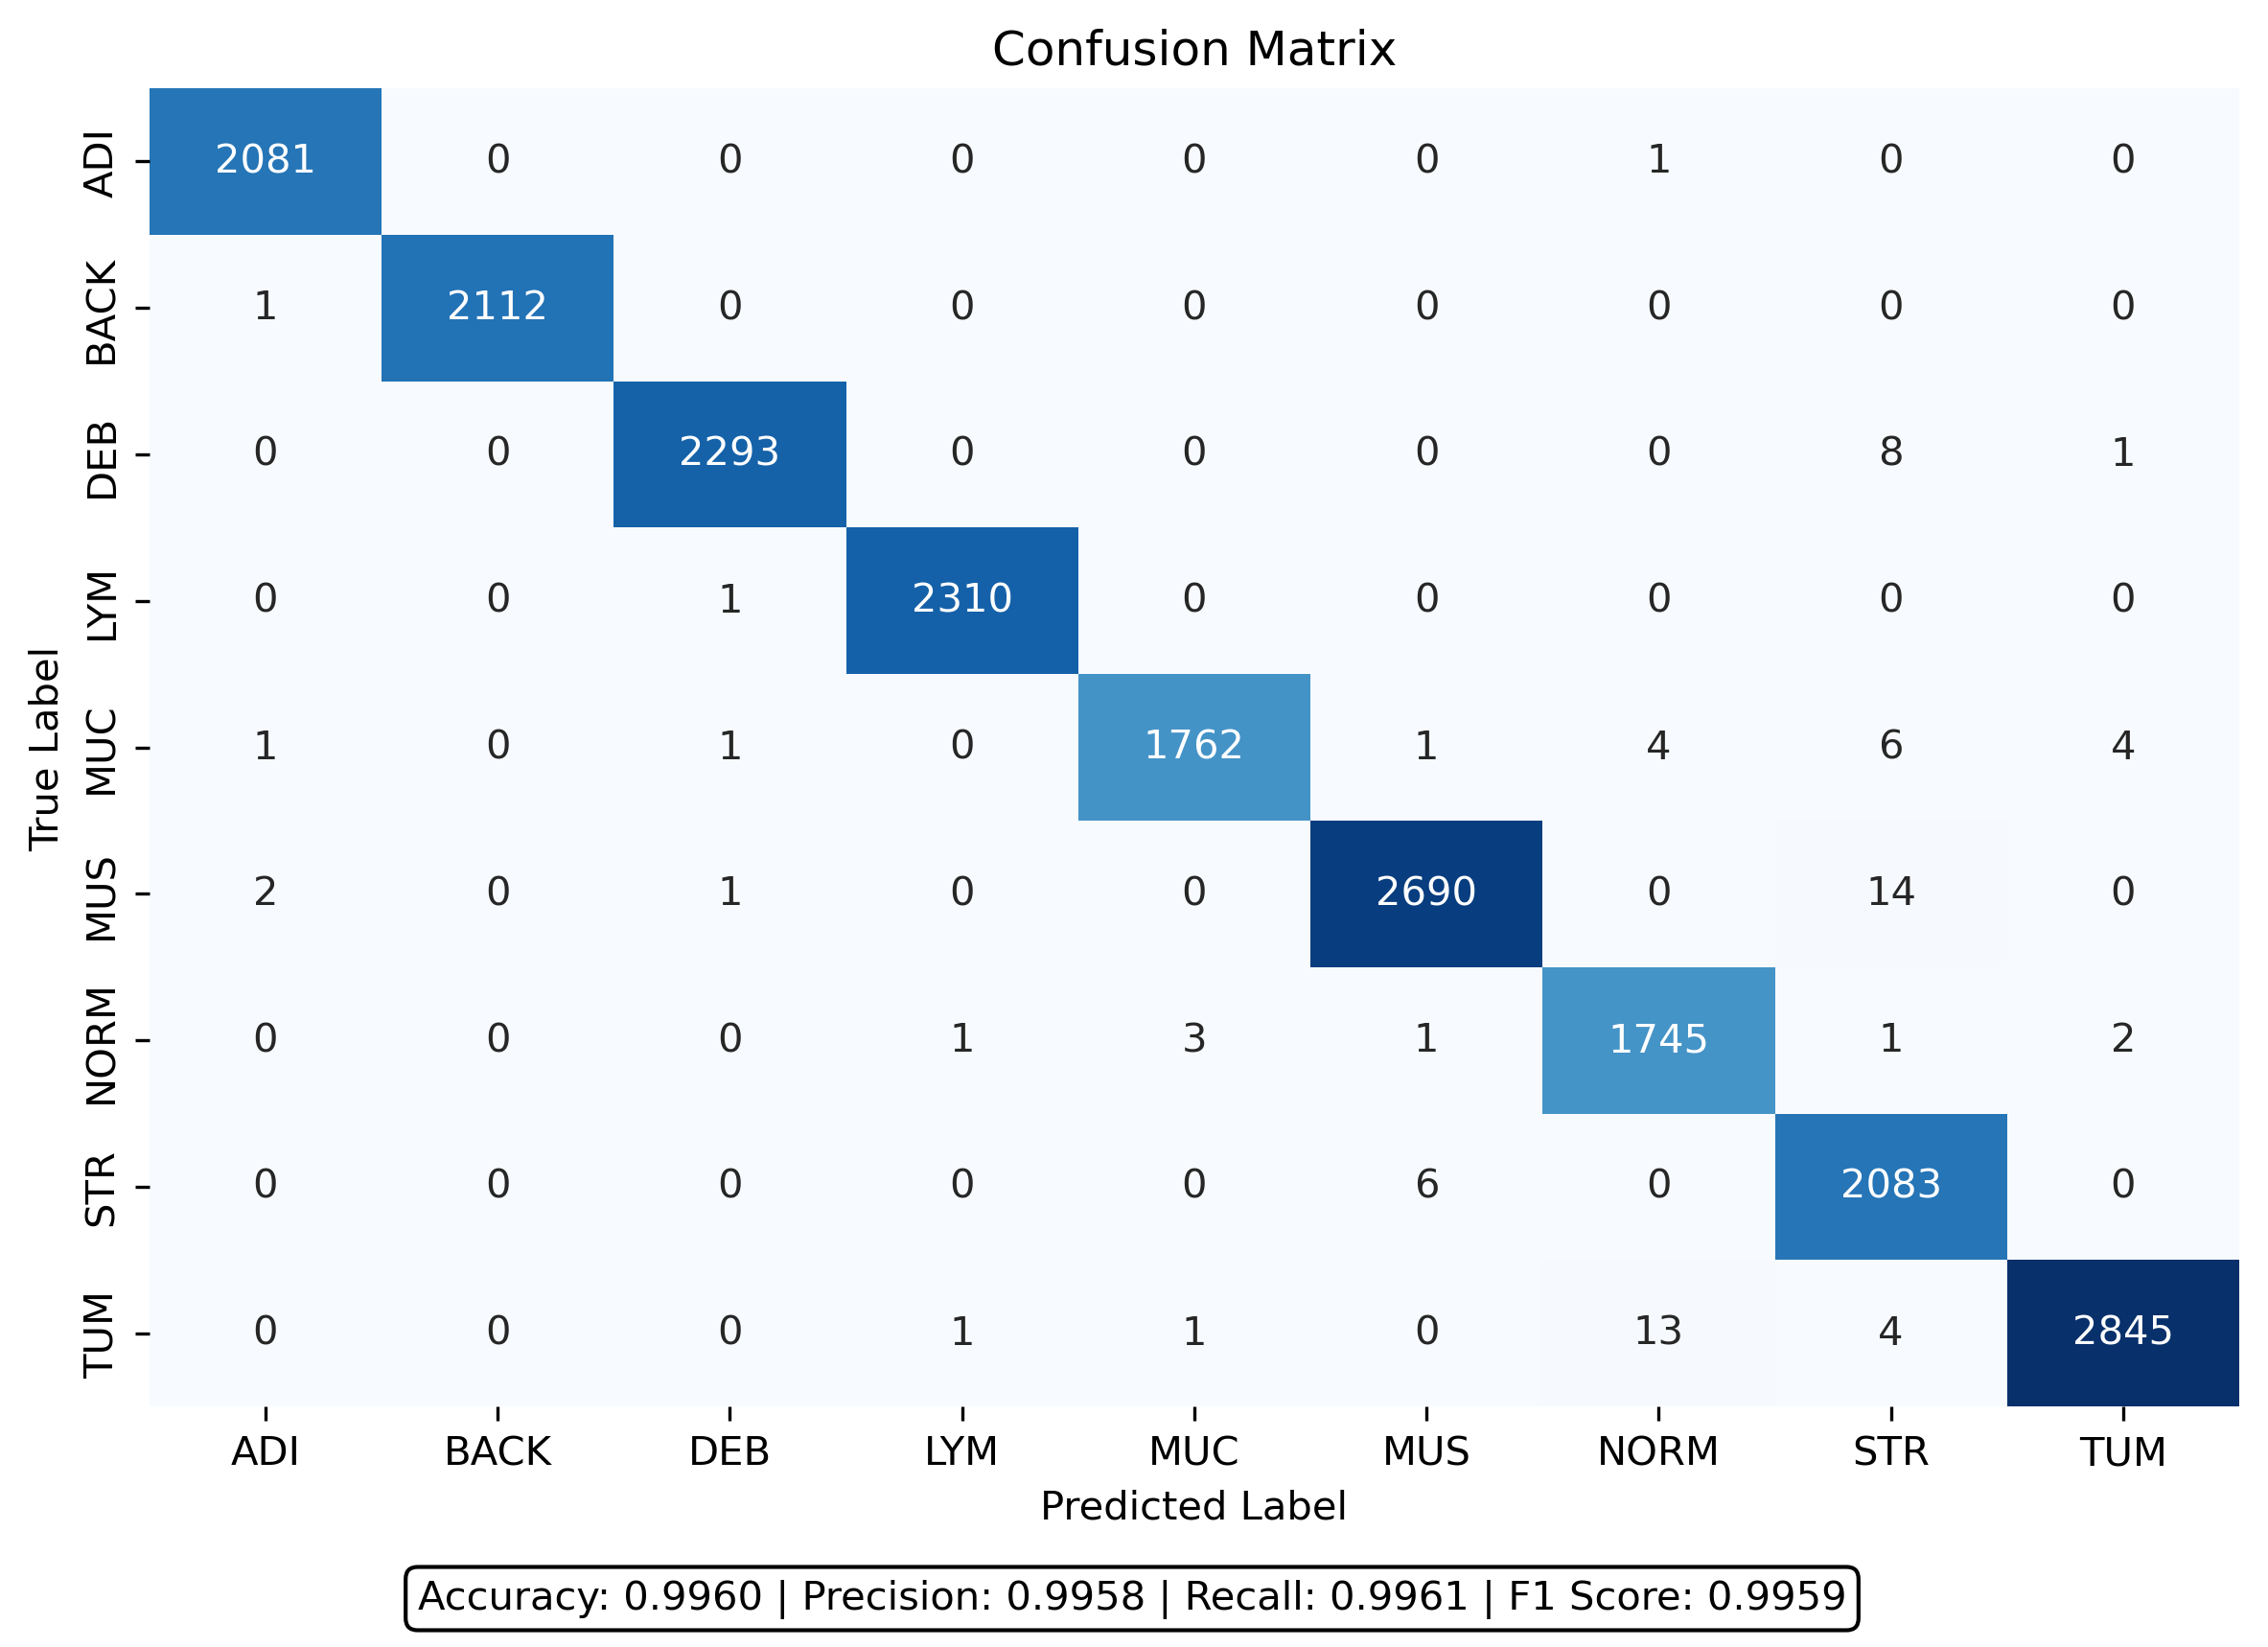
\includegraphics[width=.8\linewidth]{../runs/resnet50_experiment/figs/confusion_matrix.png}
    \caption{Confusion matrix for ResNet-50 classification.}
    \label{fig.conf_mat_resnet}
\end{figure}

\begin{figure}[H]
    \centering
    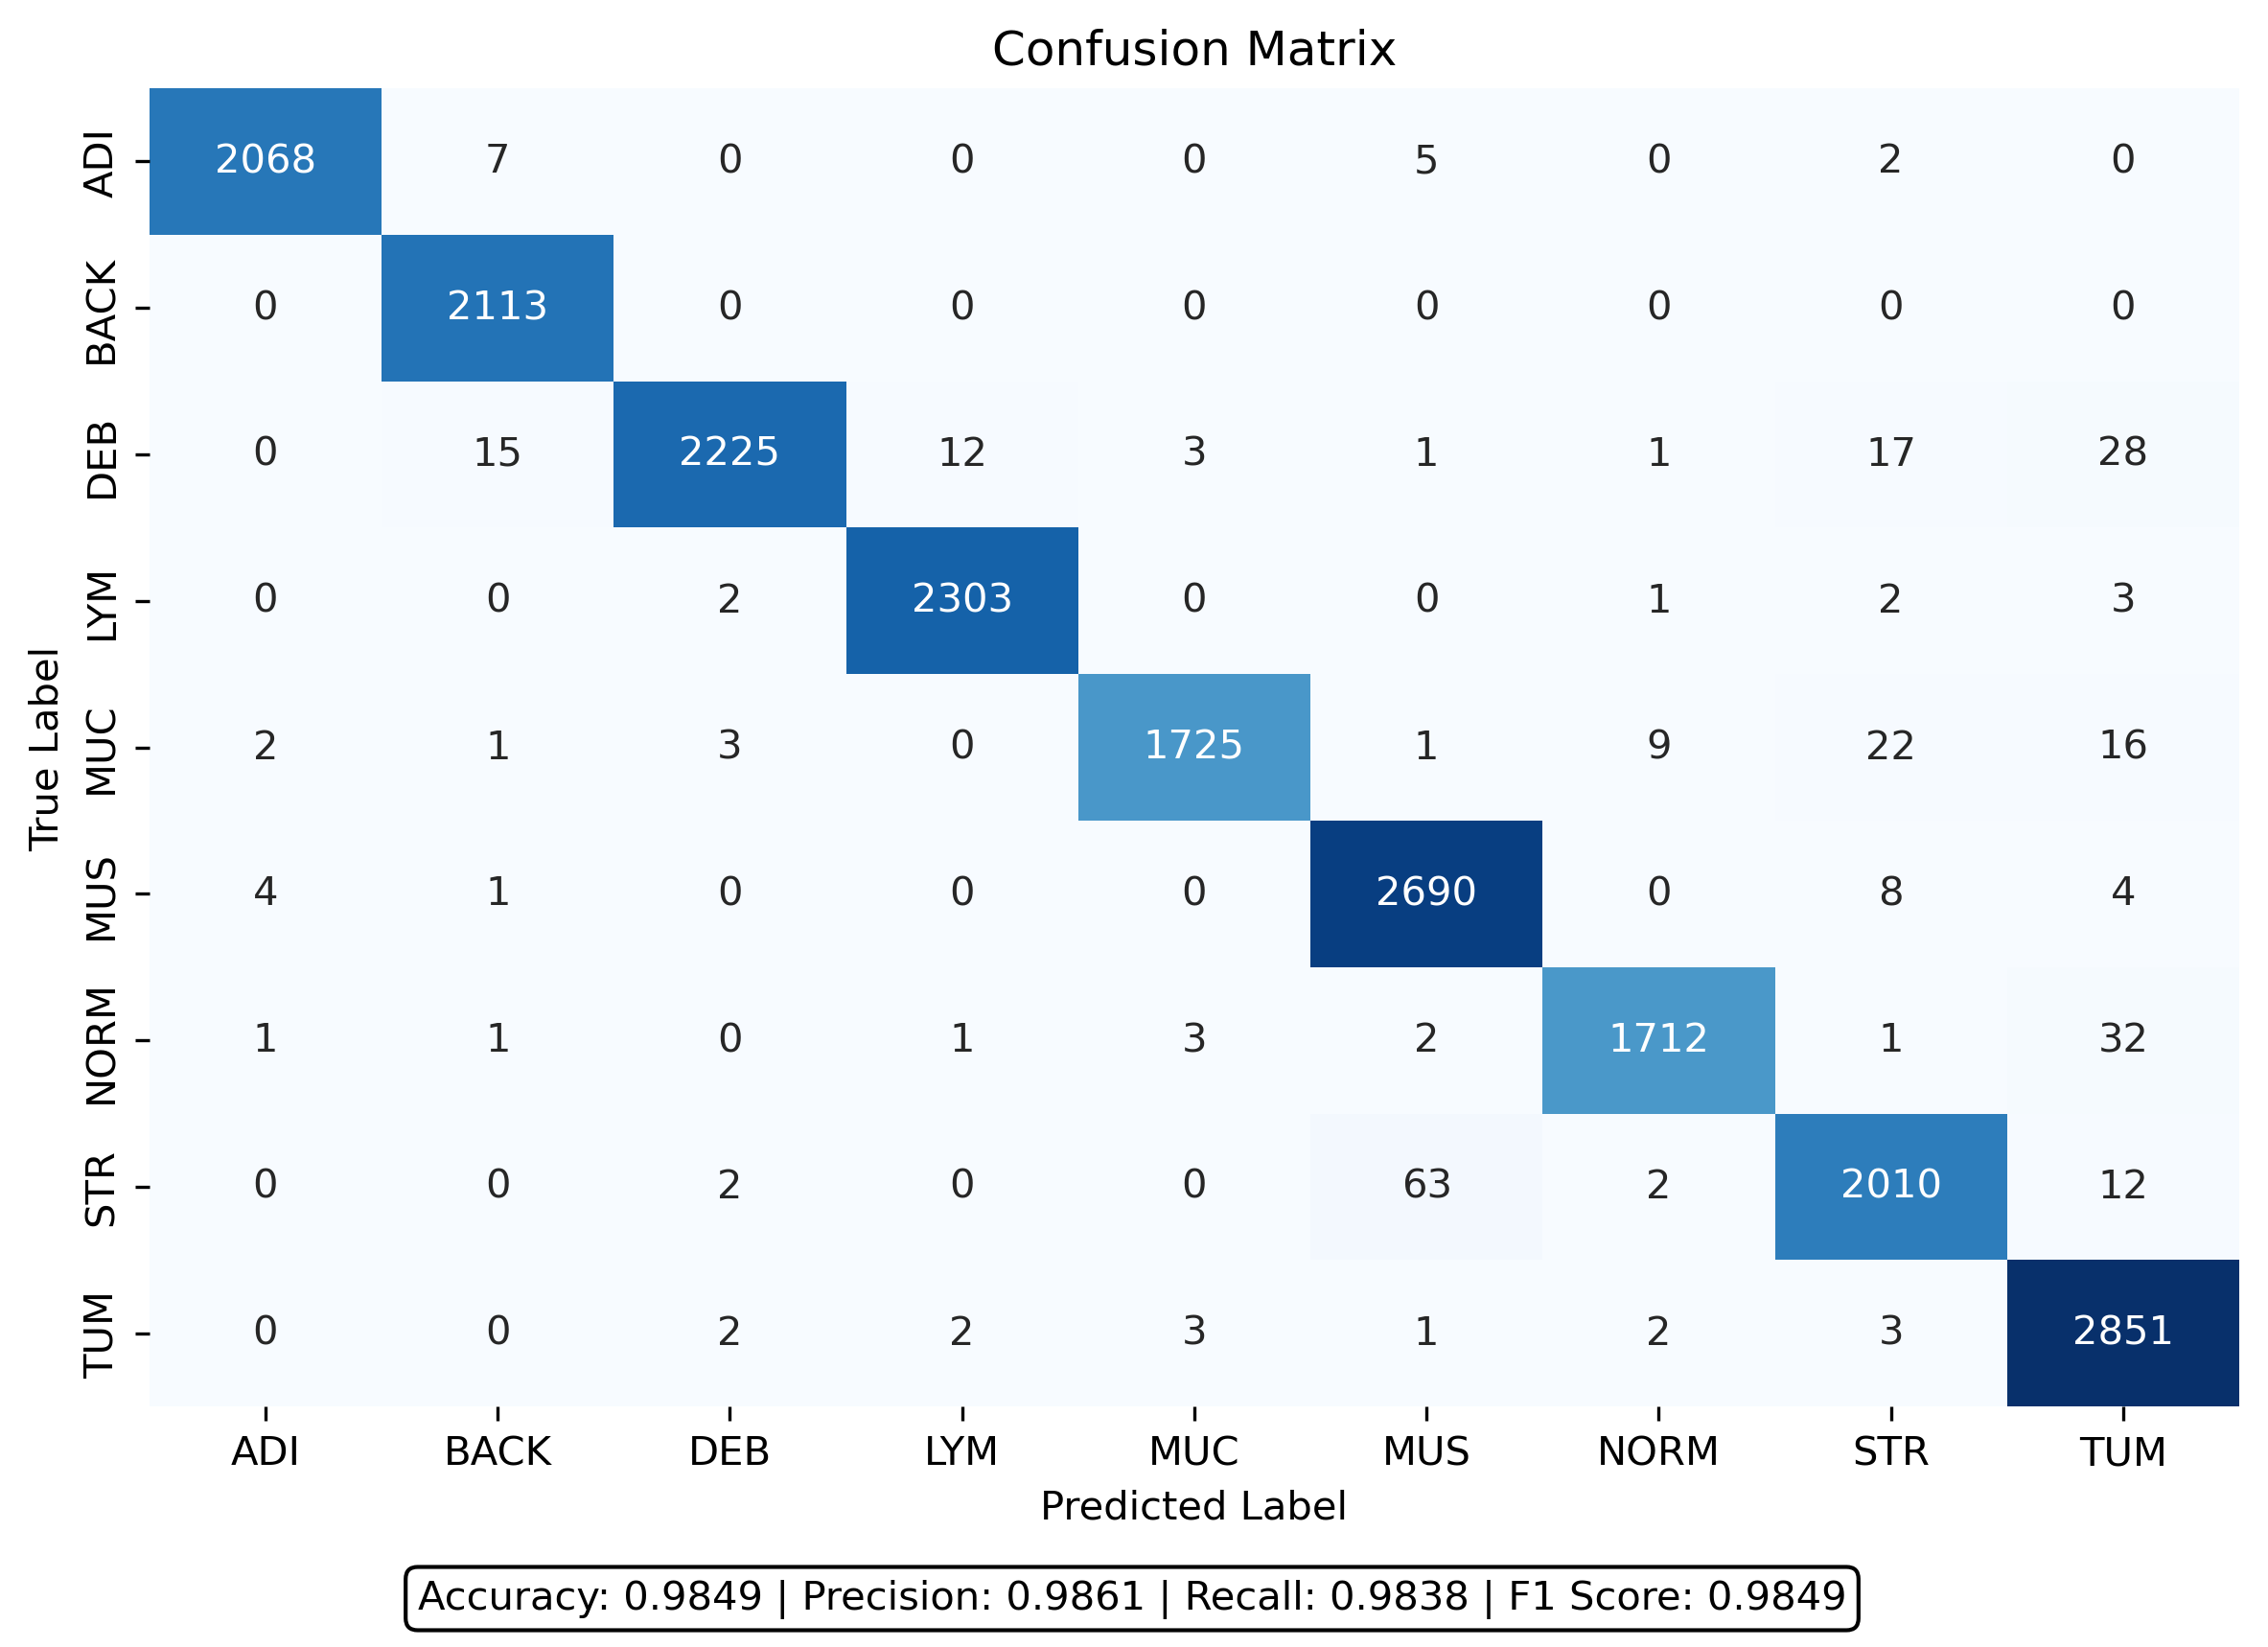
\includegraphics[width=.8\linewidth]{../runs/vgg16_experiment/figs/confusion_matrix.png}
    \caption{Confusion matrix for VGG-16 classification.}
    \label{fig.conf_mat_vgg}
\end{figure}

\begin{figure}[H]
    \centering
    \includegraphics[width=.8\linewidth]{../runs/resnet50_experiment/figs/ROC_curve.png}
    \caption{Multiclass receiver operating characteristic (ROC) curve for ResNet-50 classification.}
    \label{fig.roc_resnet}
\end{figure}

\begin{figure}[H]
    \centering
    \includegraphics[width=.8\linewidth]{../runs/vgg16_experiment/figs/ROC_curve.png}
    \caption{Multiclass receiver operating characteristic (ROC) curve for VGG-16 classification.}
    \label{fig.roc_vgg}
\end{figure}

The ResNet-50 confusion matrix (Figure \ref{fig.conf_mat_resnet}) is characterized by a near-perfect diagonal with only a handful of misclassifications distributed across morphologically related categories. Occasional errors arise between mucus (MUC), muscle (MUS), stroma (STR), and tumor epithelium (TUM), which is consistent with the visual similarity of glandular or stromal patterns in these regions. VGG-16 (Figure \ref{fig.conf_mat_vgg}) exhibits a similar but slightly noisier pattern: diagonal dominance is preserved, yet there are more off-diagonal entries, particularly involving DEB, MUC, NORM, STR, and TUM. These additional errors suggest that, although VGG-16 captures relevant local texture features, it is somewhat less robust than ResNet-50 at discriminating against fine-grained subtypes with overlapping morphology.

The ROC curves in Figures \ref{fig.roc_resnet} and \ref{fig.roc_vgg} further confirm that both CNN models rank class probabilities effectively, despite the small number of misclassifications visible in the confusion matrices. Taken together, these results show that end-to-end CNNs provide a very strong baseline on this homogeneous, stain-normalized dataset, yet they still underperform slightly relative to the Virchow2-based PatchMIL and MulticlassMLP classifiers. When considered alongside their substantially larger parameter counts and longer training times, this performance gap motivates the use of foundation-model embeddings with lightweight heads for efficient, high-accuracy histopathology classification.


\section{Discussion}
The evaluation of CNN-based and ViT-based models reveals distinct trade-offs regarding computational efficiency and feature expressiveness. Both transformer-based classifiers achieved near-perfect performance on the NCT-CRC-HE-100K dataset, with the simpler MulticlassMLP (CLS-token based) slightly outperforming the attention-based PatchMIL. This suggests that the pretrained Virchow2 embeddings already encode sufficiently rich semantic information, rendering complex aggregation mechanisms redundant for tile-level classification tasks.

In contrast, while the convolutional baselines remained competitive, with ResNet-50 reaching 99.60\% and VGG-16 reaching 98.49\%, they consistently lagged behind the ViT-based approaches. Crucially, the CNNs required computationally expensive end-to-end training to adapt to the histopathology domain \cite{kather_predicting_2019}. The ViT models, by leveraging frozen foundation model features, achieved superior results with a fraction of the trainable parameters, demonstrating that transfer learning from large-scale self-supervised models offers a more efficient alternative to traditional supervised training.

\subsection{Error Analysis}
Misclassifications across all models were primarily concentrated among morphologically similar categories, specifically stroma (STR) versus tumor epithelium (TUM). However, the ViT-based classifiers exhibited much fewer errors than VGG-16 or ResNet-50. This performance gap highlights the advantage of the transformer's global self-attention mechanism, which captures broader micro-architectural context, over the local texture bias inherent to standard CNN architectures.

\subsection{Limitations}
Despite high ROC-AUC values, these results must be interpreted within the context of the dataset's homogeneity. The current patch-level splitting strategy may allow for information leakage compared to strict patient-level or slide-level splits, potentially inflating performance metrics. Future work should prioritize evaluating generalization on heterogeneous external datasets (e.g., TCGA-BRCA) and incorporating calibration metrics to better assess clinical reliability.

% \section{Discussion}
% The performance of both PatchMIL and MulticlassMLP is consistent with recent advances in transformer-based computational pathology. Prior work on Virchow2, HistoMIL, and other large-scale ViT models reports patch-level accuracies around 94-97\%, emphasizing the strong transferability of pretrained self-supervised representations. The ability of our lightweight classifier heads to exceed these benchmark ranges highlights the advantage of additional training on foundation-model embeddings. Both transformer-based classifiers, PatchMIL and the CLS-token MulticlassMLP, achieved near-perfect performance on the NCT-CRC-HE-100K dataset. Although PatchMIL is designed to aggregate fine-grained patch information through attention weighting, the simpler MulticlassMLP slightly outperformed it. This suggests that the pretrained Virchow2 ViT-H/14 embeddings already encode sufficiently rich local and global morphological signals, reducing the marginal benefit of more complex aggregation mechanisms. The minimal accuracy difference (<0.3\%) further indicates that, under conditions of strong stain normalization and limited inter-slide variability, lightweight classifiers built on foundation-model embeddings are sufficient for high-fidelity patch-level prediction.

% The convolutional baselines also performed strongly: ResNet-50 reached an accuracy of 99.60\%, while VGG-16 achieved 98.49\%. These results confirm that CNNs remain competitive on homogeneous datasets. However, both architectures underperformed relative to PatchMIL and MulticlassMLP and required substantially larger parameter counts and longer training times. The performance gap, combined with the computational efficiency of training on a pretrained foundation model, suggests that transformer embeddings provide more expressive and transferable representations than end-to-end CNNs for histopathology image analysis.

% \subsection{Comparison with Previous Work}
% Compared with typical CNN baselines, such as ResNet-50 models reporting ∼91–93\% accuracy in earlier studies \cite{kather_predicting_2019}, our approach benefits significantly from the high transferability of foundation models. While CNN architectures achieve strong performance on the NCT dataset, they necessitate end-to-end training to adapt their features to the histopathology domain. In contrast, the robust representations of the transformer-based backbone allow us to freeze the feature extractor and train only a lightweight classifier. This results in a substantial reduction in trainable parameters compared to CNN baselines, which rely on full fine-tuning to overcome the domain gap.

% \subsection{Error Analysis and Interpretation}
% Most model errors occurred among morphologically adjacent categories, particularly stroma (STR) versus tumor epithelium (TUM) and mucus (MUC) versus tumor. These confusions are biologically interpretable: tumor-associated stroma often contains reactive fibroblasts and immune infiltrates that resemble epithelial tumor textures, while mucus-rich regions in glandular tumors exhibit visual overlap with mucinous tissue. Such cases reflect the inherent limitations of 224$\times$224 tiles, which may not fully capture the micro-architectural context required for unambiguous distinction.

% The CNN models exhibited characteristic CNN-specific error patterns. ResNet-50 showed occasional confusion among MUC, MUS, STR, and TUM, consistent with CNNs’ reliance on localized texture cues. VGG-16 exhibited broader misclassification, likely reflecting its lower representational capacity and lack of residual connections for deep refinement. These patterns contrast with the ViT-based classifiers, whose errors were fewer and more concentrated. The superior performance of the ViT-derived embeddings suggests that transformers' global self-attention enables richer modeling of contextual tissue structures, reducing reliance on narrow texture motifs and improving discrimination among fine-grained histological subtypes.

% \subsection{Limitations and Reliability}
% While the exceptionally high accuracy and ROC-AUC values demonstrate strong internal validity, several limitations warrant caution. The NCT-CRC-HE-100K dataset is highly homogeneous, and patch-level splitting may inadvertently allow tiles from the same whole slide to appear in both training and test sets. This can artificially inflate performance, especially for CNNs, which more readily learn slide-specific texture signatures. To more rigorously assess generalization, future studies should employ slide-level or patient-level splits and evaluate models on heterogeneous external datasets such as HISTAI or TCGA-BRCA.

% In addition, the absence of calibration metrics limits understanding of the models’ reliability in clinical uncertainty settings. Reporting additional measures, such as precision–recall curves or expected calibration error, would provide a more comprehensive assessment.


\section{Conclusion}
This study demonstrates that utilizing pretrained ViT-based foundation model embeddings enhances classification performance in histopathology compared to traditional end-to-end CNN architectures. Our results also indicate that the lightweight MulticlassMLP performs slightly better than the more complex PatchMIL, suggesting that the frozen CLS token from Virchow2 already captures the necessary morphological semantics for high-accuracy prediction without requiring intricate attention mechanisms. However, while this transformer-based pipeline offers a distinct advantage for rapid prototyping by drastically reducing training times, it comes with a trade-off in deployment costs due to the much larger total parameter count of the underlying foundation model and final classifier combined. Consequently, standard CNNs like ResNet-50 remain superior for large-scale, resource-constrained deployment, as their compact architectures ensure faster inference speeds and lower memory usage once fully trained.

\subsection{Contributions}
\begin{enumerate}
    \item \textbf{Tiger} was responsible for the technical implementation and the methodology. He developed the model training pipelines for both the CNN baselines (VGG-16, ResNet-50) and the ViT-based classifiers (PatchMIL, MulticlassMLP). Additionally, he drafted the Methods section, detailing the architectural specifications and experimental setup.

    \item \textbf{Estella} led the data analysis and evaluation. She compiled the experimental data to author the Results and Discussion sections, providing critical insights into the performance trade-offs between embedding strategies and interpreting the error patterns across different histopathology tissue types.

    \item \textbf{Leo} established the conceptual framework of the study. He authored the Introduction, defining the scope and motivation of the research, and synthesized the final findings in the Conclusion. He also performed comprehensive proofreading and editing to ensure the manuscript's coherence and clarity.
\end{enumerate}

\subsection{Future Work}
Future directions include:
\begin{enumerate}
    \item Evaluating cross domain performance on external datasets (e.g. HISTAI, TCGA-BRCA)
    \item Incorporating explainable AI techniques such as Grad-CAM, attention rollout, or counterfactual analysis
    \item Applying knowledge distillation or model quantization to reduce computational overhead
    \item Introducing graph-based or neighborhood-consistency modeling to capture spatial context across adjacent tiles
    \item Validating model robustness under stain, brightness, or blur perturbations
\end{enumerate}

These steps will extend the current results toward clinically reliable, generalizable, and interpretable computational pathology systems.

\label{LastPage}

% Appendix
\clearpage
\pagestyle{empty}
\section*{Appendix}
Code repo: https://github.com/zydtiger/patch-classification

% References
\clearpage
\pagestyle{empty}
\bibliographystyle{unsrt}
\begin{flushleft}
    \bibliography{CV}
\end{flushleft}

\end{document}